%
% Modelo de trabalho acadêmico monográfico (Tese de Doutorado, Dissertação de Mestrado
% ou Projeto de Qualificação) em português brasileiro e em conformidade com as normas da ABNT
%
% Documento principal
% Data: 07 de outubro de 2014
%
% *****************************************************************************
% *  Centro Federal de Educação Tecnológica de Minas Gerais - CEFET-MG        *
% *  Laboratório de Sistemas Inteligentes - LSI                               *
% *                                                                           *
% *  Autor: Henrique E. Borges <henrique@lsi.cefetmg.br>                      *
% *  Autor: Denise de Souza <densouza@gmail.com>                              *
% *  Autor: Cristiano Fraga G. Nunes <cfgnunes@gmail.com>                     *
% *  Autor: Lauro César <https://code.google.com/p/abntex2/>                  *
% *                                                                           *
% *****************************************************************************



\documentclass[
      %twoside,					% Impressão em frente (anverso) e verso. Oposto a oneside
      oneside,					% Impressão apenas no anverso. Oposto a twoside
      a4paper,					% Tamanho do papel
%   opções do pacote babel
      english,					% Idioma adicional para hifenização
      brazilian,				% O ultimo idioma indicado será o principal idioma do documento    
]{abntex2-cefetmg} 




% -----------------------------------------------------------------------------
%    Configura as citações bibliográficas conforme a norma ABNT
% -----------------------------------------------------------------------------

\usepackage[brazilian,hyperpageref]{backref}
\usepackage[alf, 
abnt-emphasize=bf, 
bibjustif, 
recuo=0cm,
abnt-doi=expand,                % Expande um endereço iniciado com doi: para http://dx.doi.org/
abnt-url-package=url,           % utiliza o pacote url
abnt-refinfo=yes,               % utiliza o estilo bibliográfico abnt-refinfo
abnt-etal-cite=3, 
abnt-etal-list=3,
abnt-thesis-year=final]{abntex2cite}	% Formata as citações bibliográficas conforme a norma ABNT


% -----------------------------------------------------------------------------
%    Pacotes utilizados 
% -----------------------------------------------------------------------------

%\usepackage[latin1]{inputenc}	% Codificação do documento (conversão automatica dos acentos)
\usepackage[utf8]{inputenc}		% Codificação do documento (conversão automatica dos acentos)
\usepackage[T1]{fontenc}		% Seleção de código de fonte
%\usepackage{times}				% Usa a fonte Times
%\usepackage{lmodern}			% Usa a fonte Latin Modern
%\usepackage{palatino}			% Usa a fonte Palatino
%\usepackage{lmodern}			% Usa a fonte Latin Modern
\usepackage{scalefnt}			% Permite redimensionar tamanho da fonte
\usepackage[scaled]{helvet}		% Usa a fonte Helvetica (default)
	\renewcommand*\familydefault{\sfdefault} 	
%\usepackage{ae,aecompl}		% Fontes de alta qualidade
\usepackage{upgreek}			% Permite inserção de letras gregas
\usepackage{latexsym}			% Permite inserção de símbolos matemáticos
\usepackage{amsfonts, amssymb, amsmath, dsfont}		% fontes e símbolos matemáticos

\usepackage{lscape}				% Permite páginas em modo "paisagem"
\usepackage{indentfirst}		% Indenta o primeiro parágrafo de cada seção.
\usepackage{microtype} 			% Melhora a justificação do documento
\usepackage{hyperref} 			% Usado para criar “hyperlinks” no PDF
%\usepackage[hyphens]{url}    	% Melhora apresentação de URLs
%\usepackage{url}              	% Melhora apresentação de URLs
\usepackage{breakurl}			% Permite quebra de linha em URLs longas
%\usepackage{balance}			% Balanceia o texto no artigo
\usepackage[bottom]{footmisc}	% Mantém as notas de rodapé sempre na mesma posição
\usepackage{verbatim}			% Permite apresentar texto tal como escrito no documento, ainda que sejam comandos Latex
%\usepackage{lettrine} 			% Lettrine é a primeira letra do início de um texto que é aumentada em relação às demais
\usepackage[pointedenum]{paralist} 		% Usado elaborar listas numeradas ou de “bullets”, aninhadas ou não 

\usepackage{graphicx}			% Inclusão de gráficos e figuras
%\usepackage{subfig}			% Permite posicionar figuras
%\usepackage{picinpar}			% Permite posicionar imagens em parágrafos
%\usepackage{psfrag}			% Inclusão de símbolos latex em figuras eps
\usepackage{tikz}	 			% Pacote para desenhos
\usepackage{color, colortbl}	% Controle das cores
\usepackage{booktabs}			% Réguas horizontais em tabelas
\usepackage{multirow, array}	% Permite tabelas com múltiplas linhas e colunas
\usepackage[algoruled, portuguese]{algorithm2e}		% Permite escrever algoritmos em português
\usepackage{float}				% Necessário para tabelas/figuras em ambiente multi-colunas
								% Devem ser, necessariamente, colocados em pontos específicos junto com [H] (e.g., \begin{table}[H])
\usepackage{subeqnarray}		% Permite subnumeracao de equações

%\usepackage{comandos} 			% Novos comandos
%\usepackage{etoolbox}	 		% Pacote para tratamento de condicionais (if-else-end \ string)
%\usepackage{ifthen}				% Pacote para tratamento de condicionais (if-else-end \ number)

%\usepackage{babel}				% Usado para definir idioma do documento e respectivas hifenizações

\usepackage{bookmark}			% Cria menu de bookmarks
%\usepackage{nomencl} 			% Usado para produzir lista de símbolos
\usepackage{makeidx}			% Usado para produzir índice remissivo (glossário)
	\makeindex 					% Compila o índice
	
%\usepackage{multind}			% Usado para produzir índices múltiplos
%\usepackage{acronym}			% Usado para produzir acrônimos
%\usepackage{bibentry}			% Permite uso de bibtex inline



%   Insere e constroi alguns elementos pré-textuais para gerar capa, folha de rosto e fe folha de aprovação

% -----------------------------------------------------------------------------
%   Arquivo: ./01-elementos-pre-textuais/capa.tex
% -----------------------------------------------------------------------------



% -----------------------------------------------------------------------------
%   ATENÇÃO:
%   Caso algum campo não se aplique ao seu documento - por exemplo, em seu trabalho
%   não houve coorientador - não comente o campo, apenas deixe vazio, assim: \campo{}
% -----------------------------------------------------------------------------



% -----------------------------------------------------------------------------
%   Dados do trabalho acadêmico
% -----------------------------------------------------------------------------

\titulo{Machine  Learning  Automated  Model  Comparison}
%\title{Title in English}
\subtitulo{ um  software  para automatizar  a  comparação  entre  métodos  de  aprendizado}
\autor{Paulo Cirino Ribeiro Neto}
\local{Belo Horizonte}
\data{Novembro de 2017}			% normalmente se usa apenas mês e ano



% -----------------------------------------------------------------------------
%   Natureza do trabalho acadêmico
%   Use apenas uma das opções: Tese (p/ Doutorado), Dissertação (p/ Mestrado) ou
%   Projeto de Qualificação (p/ Mestrado ou Doutorado), Trabalho de Conclusão de
%   Curso (Graduação)
% -----------------------------------------------------------------------------

\projeto{Trabalho de Conclusão de Curso}



% -----------------------------------------------------------------------------
%   Título acadêmico
%   Use apenas uma das opções:
%	Se a natureza for Tese, coloque Doutor
%	Se a natureza for Dissertação, coloque Mestre
%	Se a natureza for Projeto de Qualificação, coloque Mestre ou Doutor conforme o caso
%   Se a natureza for Trabalho de Conclusão de Curso, coloque Bacharel
% -----------------------------------------------------------------------------

\tituloAcademico{Doutor}



% -----------------------------------------------------------------------------
%   Área de concentração e linha de pesquisa
%	OBS: indique o nome da área de concentração e da linha de pesquisa do Programa de Pós-graduação
%   nas quais este trabalho se insere
%   Se a natureza for Trabalho de Conclusão de Curso, deixe ambos os campos vazios
% -----------------------------------------------------------------------------


%\areaconcentracao{Aprendizado de Máquina}
%%\linhapesquisa{Sistemas Inteligentes}



% -----------------------------------------------------------------------------
%   Dados da instituicao
%   OBS: a logomarca da instituiçã deve ser colocada na mesma pasta que foi colocada o documento
%   principal com o nome de "logoInstituicao". O formato pode ser: pdf, jpf, eps
%   Se a natureza for Trabalho de Conclusão de Curso, coloque em "programa' o nome do curso de graduação
% -----------------------------------------------------------------------------

\instituicao{Universidade Federal de Minas Gerais}
\programa{Engenharia de Sistemas}
%\programa{Curso de Engenharia de Computação}
\logoinstituicao{0.2}{logoInstituicao}                  % \logoinstituicao{<escala>}{<nome do arquivo>}



% -----------------------------------------------------------------------------
%   Dados do(s) orientador(es)
% -----------------------------------------------------------------------------

\orientador{Antônio de Pádua Braga}
%\orientador[Orientadora:]{Nome da orientadora}
\instOrientador{Universidade Federal de Minas Gerais}

\coorientador{Gustavo Rodrigues Lacerda Silva}
%\coorientador[Coorientadora:]{Nome da coorientadora}
\instCoorientador{Universidade Federal de Minas Gerais}



% -----------------------------------------------------------------------------
%   Arquivo: ./01-elementos-pre-textuais/folhaRosto.tex
% -----------------------------------------------------------------------------



% -----------------------------------------------------------------------------
%   Trabalho de Conclusão de Curso
% -----------------------------------------------------------------------------

\preambulo{{\imprimirprojeto} apresentado ao Curso de Engenharia de Sistemas da Universidade Federal de Minas Gerais, como requisito parcial para a obtenção do título de {\imprimirtituloAcademico} em Engenharia de Sistemas.}



% -----------------------------------------------------------------------------
%   Projeto de qualificação de Mestrado ou Doutorado
% -----------------------------------------------------------------------------

%\preambulo{{\imprimirprojeto} apresentado ao Programa de \mbox{Pós-graduação} em Modelagem Matemática e Computacional do Centro Federal de Educação Tecnológica de Minas Gerais, como requisito parcial para a obtenção do título de {\imprimirtituloAcademico} em Modelagem Matemática e Computacional.}



% -----------------------------------------------------------------------------
%   Dissertação de Mestrado
% -----------------------------------------------------------------------------

%\preambulo{{\imprimirprojeto} apresentada ao Programa de \mbox{Pós-graduação} em Modelagem Matemática e Computacional do Centro Federal de Educação Tecnológica de Minas Gerais, como requisito parcial para a obtenção do título de {\imprimirtituloAcademico} em Modelagem Matemática e Computacional.}



% -----------------------------------------------------------------------------
%   Tese de Doutorado
% -----------------------------------------------------------------------------

%\preambulo{{\imprimirprojeto} apresentada ao Programa de \mbox{Pós-graduação} em Modelagem Matemática e Computacional do Centro Federal de Educação Tecnológica de Minas Gerais, como requisito parcial para a obtenção do título de {\imprimirtituloAcademico} em Modelagem Matemática e Computacional.}




% -----------------------------------------------------------------------------
%   Edite este arquivo comentando as linhas que não se aplicam ao tipo de documento acadêmico pretendido.
% -----------------------------------------------------------------------------
% -----------------------------------------------------------------------------
%   Arquivo: ./01-elementos-pre-textuais/folhaAprovacao.tex
% -----------------------------------------------------------------------------



\textopadraofolhadeaprovacao{Esta folha deverá ser substituída pela cópia digitalizada da folha de aprovação fornecida pelo Programa de Pós-graduação.}



% -----------------------------------------------------------------------------
%  Este documento foi mantido apenas para preservar a paginação do trabalho acadêmico
%  final, após a inserção da folha de arpovação fornecida pelo programa.
% -----------------------------------------------------------------------------





% -----------------------------------------------------------------------------
%   Configurações de aparência do PDF final
% -----------------------------------------------------------------------------

\definecolor{blue}{RGB}{41,5,195}	% Altera o aspecto da cor azul

\makeatletter
\hypersetup{
	portuguese,
    colorlinks=true,       	% true: “links” coloridos; false: “links” em caixas de texto
	linkcolor=blue,			% Define cor dos “links” internos”
	citecolor=blue,			% Define cor dos “links” para as referências bibliográficas
	filecolor=blue,			% Define cor dos “links” para arquivos
	urlcolor=blue, 			% Define a cor dos “hiperlinks”
	breaklinks=true,
	pdftitle={\@title},
	pdfauthor={\@author},
%	pdfsubject={\imprimirpreambulo},
	pdfkeywords={abnt, latex, abntex, abntex2}
}
\makeatother



% -----------------------------------------------------------------------------
%   Hifenização de palavras não constantes do dicionário
% -----------------------------------------------------------------------------

\hyphenation{
		qua-dros-cha-ve
		Bras-nett
		Kat-sa-gge-los
}



% -----------------------------------------------------------------------------
%   Inclui todos os arquivos do trabalho acadêmico
% -----------------------------------------------------------------------------

\begin{document}

\frenchspacing				%   Retira o espaço extra desnecessário nas frases

%   Gera e imprime alguns elementos pré-textuais: capa, folha de rosto e folha de aprovação

\pretextual
\imprimircapa 											% Comando para imprimir Capa
\imprimirfolhaderosto{} 								% Comando para imprimir Folha de rosto
\imprimirfolhadeaprovacao{} 							% Comando para imprimir Folha de aprovação

%   Insere os demais elementos pré-textuais

% -----------------------------------------------------------------------------
%   Arquivo: ./01-elementos-pre-textuais/dedicatoria.tex
% -----------------------------------------------------------------------------



\begin{dedicatoria}

Dedico esse trabalho à meus familiares, amigos, colegas e professores.


\end{dedicatoria}

		% Dedicatória
%%% -----------------------------------------------------------------------------
%   Arquivo: ./01-elementos-pre-textuais/agradecimentos.tex
% -----------------------------------------------------------------------------



\begin{agradecimentos}

Edite e coloque aqui os agradecimentos às pessoas e/ou instituições que contribuíram para a realização do trabalho.

É obrigatório o agradecimento às instituições de fomento à pesquisa que financiaram total ou parcialmente o trabalho, inclusive no que diz respeito à concessão de bolsas.


\end{agradecimentos}
	% Agradecimentos
% -----------------------------------------------------------------------------
%   Arquivo: ./01-elementos-pre-textuais/epigrafe.tex
% -----------------------------------------------------------------------------



\begin{epigrafe}

\textit{``The only excuse for making a useless thing is that one admires it intensely.''}
(Oscar Wilde, prefácio, O retrato de Dorian Gray)
\end{epigrafe}



% -----------------------------------------------------------------------------
%   Edite o texto acima para inserir uma epígrafe de sua preferência
% -----------------------------------------------------------------------------
			% Epígrafe
% -----------------------------------------------------------------------------
%   Arquivo: ./01-elementos-pre-textuais/resumoPt.tex
% -----------------------------------------------------------------------------



\begin{resumo}

O  tema  desse trabalho  de  conclusão  de  curso  é  a criação de um software  para  automatizar testes  de  modelos  de  aprendizado  de  máquina. 

Ao  fim  do  projeto,  existirá  um  software, escrito na linguagem de programação R, capaz  de  comparar  modelos  de  aprendizado  de máquina  consagrados  na  literatura com  modelos  criados  pelo  usuário.  O  software  fará  o tratamento  das  bases  de  dados  padrões,  suas  chamadas  e  os  testes  estatísticos  de qualidade e tempo para os problemas de classificação, regressão e clusterização.

Será discutido nesse trabalho, o impacto social de software livre e os aspectos técnicos e definições matemáticas do aprendizado supervisionado e não supervisionado.

\textbf{Palavras-chave}: Software Livre. Aprendizado de Máquina. Linguagem R. Teste de Modelos.

 

\end{resumo}



% -----------------------------------------------------------------------------
%   Escolha de 3 a 6 palavras ou termos que descrevam bem o seu trabalho. As palavras-chaves são utilizadas para indexação.
%   A letra inicial de cada palavra deve estar em maiúsculas. As palavras-chave são separadas por ponto.
% -----------------------------------------------------------------------------
			% Resumo na língua vernacular
% -----------------------------------------------------------------------------
%   Arquivo: ./01-elementos-pre-textuais/resumoEn.tex
% -----------------------------------------------------------------------------



\begin{resumo}[Abstract]
The theme of this work is the creation of a software capable of automating machine learning models testing.

At the end of the project, there will be a software written in the R programming language, capable of comparing established machine learning model  with ones created by the user. The software will make standard database treatments, create function calls for testing, and define statistical tests routines of bolth quality and time for classification, regression and clustering problems.

The discussion of social impact of free software and the technical and mathematical aspects of supervised and unsupervised learning, will also be part of the project.

\textbf{Keywords}: Free Software. Machine Learning. R programming Language. Model Testing.


\end{resumo}



% -----------------------------------------------------------------------------
%   O restante da formatação deve manter-se igual ao do reusmo em português, i.e, um único parágrafo.
% -----------------------------------------------------------------------------
			% Resumo em língua inglesa
% -----------------------------------------------------------------------------
%   Arquivo: ./01-elementos-pre-textuais/listaFiguras.tex
% -----------------------------------------------------------------------------



\pdfbookmark[0]{\listfigurename}{lof}
\listoffigures*
\cleardoublepage



% -----------------------------------------------------------------------------
%   Este arquivo não necessita de ser editado. A lista é gerada automaticamente.
% -----------------------------------------------------------------------------		% Lista de figuras
% -----------------------------------------------------------------------------
%   Arquivo: ./01-elementos-pre-textuais/listaTabelas.tex
% -----------------------------------------------------------------------------



\pdfbookmark[0]{\listtablename}{lot}
\listoftables*
\cleardoublepage



% -----------------------------------------------------------------------------
%   Este arquivo não necessita de ser editado. A lista é gerada automaticamente.
% -----------------------------------------------------------------------------		% Lista de tabelas
%% -----------------------------------------------------------------------------
%   Arquivo: ./01-elementos-pre-textuais/listaQuadros.tex
% -----------------------------------------------------------------------------



\pdfbookmark[0]{\listofquadrosname}{loq}
\listofquadros*
\cleardoublepage



% -----------------------------------------------------------------------------
%   Este arquivo não necessita de ser editado. A lista é gerada automaticamente.
% -----------------------------------------------------------------------------		% Lista de quadros
% -----------------------------------------------------------------------------
%   Arquivo: ./01-elementos-pre-textuais/listaAlgoritmos.tex
% -----------------------------------------------------------------------------



\newcommand{\algoritmoname}{Algoritmo}
\renewcommand{\listalgorithmcfname}{Lista de Algoritmos}

\floatname{algocf}{\algoritmoname}
\newlistof{listofalgoritmos}{loa}{\listalgoritmoname}
\newlistentry{algocf}{loa}{0}

\counterwithout{algocf}{chapter}
\renewcommand{\cftalgocfname}{\algoritmoname\space}
\renewcommand*{\cftalgocfaftersnum}{\hfill--\hfill}

\pdfbookmark[0]{\listalgorithmcfname}{loa}
\listofalgorithms
\cleardoublepage



% -----------------------------------------------------------------------------
%   Este arquivo não necessita de ser editado. A lista é gerada automaticamente.
% -----------------------------------------------------------------------------	% Lista de algoritmos
% -----------------------------------------------------------------------------
%   Arquivo: ./01-elementos-pre-textuais/listaSiglas.tex
% -----------------------------------------------------------------------------



\begin{siglas}
	%\item[ABNT] Associação Brasileira de Normas Técnicas
	%\item[UFMG] Universidade Federam de Minas Gerais
	%\item[TCC] Trabalho de Conclusão de Curso
	
	%% Free Software
	\item[API] \textit{Application Program Interface}
	\item[GNU] \textit{GNU's Not Unix}
	\item[GPL] \textit{General Public License }
	\item[MIT] \textit{ Massachusetts Institute of Technology }
	\item[BSD] \textit{Berkeley Software Distribution}
	\item[NSA] \textit{National Security Agency}
	%\item[SO] Sistema Operacional
	\item[CRAN] \textit{Comprehensive R Archive Network}
	
	\item[CPU] \textit{Central Processing Unit}
	\item[GPU] \textit{Graphical Processing Unit}
	\item[HTTP] \textit{Hypertext Transfer Protocol}
	%\item[POO] Programação Orientada à Objetos
	%% Aprendizado de Maquina
	\item[RNA] Redes Neurais Artificiais
	%\item[ML] \textit{Machine Learning}
	\item[KNN] \textit{K Nearest Neighbours}
	\item[RNN] \textit{Rede Neural Artificial}
	\item[MLP]  \textit{Multilayer Perceptron }
	%\item[PCA] \textit{Principal Component Analasys}
	\item[SVM]  \textit{Support Vector Machines }
	
	
\end{siglas}



% -----------------------------------------------------------------------------
%   Edite a lista acima para definir "todos" os acrônimos e siglas utilizados neste trabalho
% -----------------------------------------------------------------------------
		% Lista de abreviaturas e siglas
% -----------------------------------------------------------------------------
%   Arquivo: ./01-elementos-pre-textuais/listaSimbolos.tex
% -----------------------------------------------------------------------------



\begin{simbolos}
	\item[$ \Gamma $] Letra grega Gama
	\item[$ \lambda $] Comprimento de onda
	\item[$ \in $] Pertence


\end{simbolos}



% -----------------------------------------------------------------------------
%   Edite a lista acima para definir "todos" os símbolos utilizados neste trabalho
% -----------------------------------------------------------------------------
		% Lista de símbolos
% -----------------------------------------------------------------------------
%   Arquivo: ./01-elementos-pre-textuais/sumario.tex
% -----------------------------------------------------------------------------



\pdfbookmark[0]{\contentsname}{toc}
\tableofcontents*
\cleardoublepage



% -----------------------------------------------------------------------------
%   Este arquivo não necessita de ser editado. O sumário é gerado automaticamente.
% -----------------------------------------------------------------------------			% Sumário

%   Insere os elementos textuais
\textual
% -----------------------------------------------------------------------------
%   Arquivo: ./02-elementos-textuais/introducao.tex
% -----------------------------------------------------------------------------

\chapter{Introdução}
\label{chap:introducao}

\section{Justificativa}
\label{sec:justificativa}
Um dos principais objetivos de softwares é auxiliar os usuários nos trabalhos com sistemas computacionais. Uma das formas de atingir esse objetivo é automatizando tarefas rotineiras, repetitivas, desinteressantes e que consomem muito tempo, liberando as pessoas para tarefas mais importantes \cite{Zambiasi2012UmaAA}. 

Uma parte fundamental no ciclo do desenvolvimento de novos algorítimos em aprendizado de máquina é o processo de \textit{benchmarking}. Esse procedimento consiste na comparação do novo método com outros modelos, além, é claro, de testes estatísticos que permitam extrair conclusões quantitativas e qualitativas.

Realizar \textit{benchmarking} pode se tornar uma tarefa repetitiva, trabalhosa e consequentemente cara. O engenheiro precisa implementar todos os métodos padrões, baixar e pré-processar todas as bases de testes, definir o planejamento e análise dos experimentos, e por fim, realizar testes estatísticos e desenhos gráficos para que seja possível extrair suas conclusões.

Dessa forma, a automatização da tarefa de \textit{benchmarking} seria benéfica ao engenheiro no sentido de economizar tempo para realizar tarefas mais importantes. Além disso, uma rotina de teste padronizada é interessante pois faz com que seja possível a comparação de estudos feitos separadamente.


\section{Objetivo}
\label{sec:objetivo}
Esse trabalho tem como objetivo a criação de um software, que seja capaz de automatizar a tarefa de \textit{benchmarking} para o teste de novos modelos de aprendizado de máquina. 

O projeto será executado na forma de pacote aberto, licença GNU GPLv3, da linguagem de programação estatística R. O pacote será implementado utilizando a própria linguagem R, sua API para $C$ e $C++$ e outros pacotes livres feitos pela comunidade.

Ao fim do ciclo de desenvolvimento, o pacote deverá ser capaz de comparar modelos para tarefas de classificação, clusterização e regressão desenvolvidos pelos usuários com diversos modelos já presentes no pacote.  O usuário poderá fornecer as bases de dados de testes ou utilizar as bases do pacote. O pacote deverá fornecer também a opção de testes estatísticos e visualizações dos resultados.

Após a conclusão do projeto, ele será enviado para publicação no repositório CRAN e submetido ao \textit{The R Journal}, um periódico para divulgação de pacotes feitos pela comunidade R.


\section{Organização do trabalho}
\label{sec:organizacaoTrabalho}

O trabalho está estruturado de forma que o capítulo \ref{chap:SoftwareLivre} tem como objetivo contextualizar e discutir os aspectos sociais e culturais do software livre, bem como falar brevemente da história desse movimento e das suas definições de liberdades sociais.

O Capítulo \ref{chap:RProgrammingLanguage}, discutirá sobre a linguagem de programação R, como ela está inserida dentro do movimento de software livre e como ela está organizada. 

Os capítulos \ref{chap:MachineLearning} e \ref{chap:testStatistics} discutirão, de forma sucinta, os conceitos de aprendizado de máquina e de estatísticas de testes que são as bases da implementação do software. 

Por fim, o capítulo \ref{chap:TheRPackage} abordará os casos de uso do projeto de software.

Nesse trabalho não serão discutidas as métricas e modelos que serão implementados, e tampouco as questões técnicas do projeto que serão abordadas no texto da disciplina de TCC II .
	
% -----------------------------------------------------------------------------
%   Arquivo: ./02-elementos-textuais/trabalhosRelacionados.tex
% -----------------------------------------------------------------------------



\chapter{Software livre}
\label{chap:SoftwareLivre}

\section{Definição de Software Livre}

A definição de software livre apresenta os critérios para determinar se um programa de software é qualificado como livre. Essa definição pode mudar conforme o momento histórico, mas atualmente é definida pela GNU como : \textit{software que os usuários têm a liberdade de executar, copiar, distribuir, estudar, alterar e melhorar} \cite{Inc2012} . 

Nesse contexto, o conceito de livre diz respeito à "liberdade de expressão", e não à gratuidade \cite{Williams}. Com essas liberdades, os usuários, tanto individualmente quanto coletivamente, controlam o programa e o que ele pode fazer. Quando os usuários não controlam o programa, chamamos ele de programa \textit{não livre} ou \textit{proprietário} \cite{Inc2012}. 

Em linhas gerais, um software livre deve, obrigatoriamente, obedecer a quatro liberdades \cite{Inc2012, Williams, Lessig2002} :
\begin{compactenum}
	\item A liberdade de executar o programa como desejar, para qualquer propósito;
	\item A liberdade de estudar como funciona o programa e mudá-lo para que ele faça a sua computação como você deseja;
	\item A liberdade de redistribuir cópias para que você possa ajudar seu vizinho;
	\item A liberdade de distribuir cópias de suas versões modificadas para outros.
\end{compactenum}

Naturalmente, essas liberdades estão relacionadas às informações divulgadas entre desenvolvedor e usuário. A liberdade \textbf{2}, por exemplo, implica na necessidade de o desenvolvedor divulgar abertamente o código fonte de um software e permitir que esse seja modificado \cite{Inc2012}. Além disso, é obvio que para os usuários terem a liberdade de decidir sobre sua computação, o software livre, por sua vez, não pode utilizar nenhum código \textit{não livre}.

É importante notar que não existem, nessas liberdades, quaisquer limitações relacionadas ao uso comercial do software. Isso significa que empresas podem cobrar pelo uso do software em versões modificadas ou não.

Além das liberdades básicas de um software livre, existem as licenças de uso. Cada licença específica, restringe ou garante mais liberdades sobre o software, sem afetar as quatro fundamentais. De forma forma geral, existem quatro famílias de licenças : \textit{Permissiva},  \textit{Fracamente Protetiva},  \textit{Fortemente Protetiva} e \textit{Protetiva de Rede} \cite{Williams}. 

\section{História do software livre}
O surgimento do movimento de software livre está altamente atrelado à academia e ao desenvolvimento dos sistemas operacionais UNIX, GNU e Linux.

O UNIX tem suas origens na \textit{joint venture}, lançada no final da década de 1960 pela \textit{Bell Labs} e MIT para criar um novo sistema operacional chamado \textit{Multics} \cite{tozzi2017fun}. Utilizando o conhecimento adquirido nesse projeto, alguns dos programadores desenvolveram, paralelamente, um sistema operacional para oferecer mais flexibilidade aos usuários, nomeado UNIX. 

Em 1975, Ken Thompson juntamente com Bill Joy e Chuck Haley, começaram a distribuir uma versão \textit{open source} do UNIX chamada BSD. No ano seguinte, o lançamento de uma edição revista foi denominada 2BSD \cite{tozzi2017fun}.

No ano de 1984, o programador Richard Stallman fundou o Projeto GNU. A GNU GPL permitia aos usuários modificar o código e distribuir a versão melhorada sob a mesma licença. O sistema operacional GNU não tinha um \textit{kernel}, até que em 1991, Linus Torvalds desenvolveu o \textit{kernel} do Linux que foi integrado no sistema operacional GNU em 1992 \cite{tozzi2017fun}.

Nos anos seguintes, foram introduzidas versões, comerciais e aprimoradas, do sistema operacional Linux por fornecedores como \textit{Red Hat}, \textit{Mandriva} e \textit{Novell}.

Com a criação de sistemas operacionais que poderiam ser utilizados com total liberdade, surgiu então uma demanda por \textit{software} livres que funcionassem nesses ambientes. Da mesma forma que a comunidade se juntou para aprimorar a base do \textit{kernel} do Linux, eles se juntaram e fizeram os mais diversos \textit{software} para atender essa demanda. 

Nos dias atuais existem inúmeras comunidades que fazem os mais variados tipos de softwares utilizando os mesmos princípios criados por Richard Stallman. Os \textit{software} livres difundiram na sociedade, e hoje são peças fundamentais para infraestrutura computacional, periféricos, celulares e virtualmente qualquer outro dispositivo computacional.

\section{A importância social do software livre}
Atualmente, os softwares livres são fundamentais principalmente em três áreas sociais: à proteção da liberdade individual, ao avanço da computação e à acessibilidade da educação e conhecimento.

\subsection{Software livre à favor da proteção da liberdade individual}
Uma celebre frase da comunidade de software livre diz, 'Os softwares não livres, onde o usuários não controlam o programa, o programa controla os usuários' \cite{Williams}. 

Essa frase, resume uma preocupação crescente com o software proprietário, a de que sempre há   alguma entidade, que controla o programa e através dele, exerce poder sobre seus usuários. 

Esse poder é enxergado por alguns como uma afronte ao direito de privacidade do indivíduo. Hoje, serviços de busca e redes sociais, utilizam dos dados de navegação para gerar propagandas sob medidas.  Muitas pessoas, consideram a forma que essas empresas manipulam as informações como uma forma de censura e venda de informação confidencial. 

Em alguns casos, empresas que desenvolvem softwares proprietários foram ligadas a escândalos onde propositalmente construíram \textit{backdoors} em seus produtos que dão acesso a informações sem as devidas permissões dos usuários. Um exemplo é o caso do \textit{ Kindle}, que possui uma \textit{backdoor} que permite apagar livros \cite{GNUOperatingSystem} .

Um outro senário onde é importante que o software seja livre, é para proteger os usuários de acesso externo indesejado. Um exemplo disso é o caso do ex analista da NSA \cite{Tate2013}, Edward Joseph Snowden, que em junho de 2013, revelou como a agência americana utilizava de falhas de seguranças, propositais ou não, para espiar na população mundial. 

O principio que o software livre protege a liberdade Individual, contra empresas mau intencionadas ou governos abusivos, é que quando o código de um programa é aberto, a comunidade pode ver oque ele faz e testar todas as falhas que o mesmo possa ter \cite{GNUOperatingSystem}.

\subsection{Software livre à favor do avanço da computação}
Após a construção dos sistemas operacionais livres, surgiram varias distribuições e variações, cada qual para atender um nicho. Esses avanços, tornaram possível que hoje, os sistemas operacionais baseados no Linux e UNIX dominassem o setor de infra estrutura computacional. Possibilitando que empresas e órgãos governamentais customizassem esses \textit{software} para criar soluções específicas para suas necessidades, que por sua vez não são necessariamente livres.

Essa abordagem se tornou tão prática que, dados da \citeonline{W3Techs} e \citeonline{Top500project2017}, mostram que esses sistemas operacionais são utilizados em $66.8\%$ de todos os servidores públicos de internet e $99.88\%$ dos supercomputadores do mundo. 

A ultima grande plataforma que popularizou a utilização do Linux foi o sistema operacional Android.  Construído inicialmente para ser um software de telefones celulares, esse sistema operacional criado com base no \textit{kernel} do Linux, se espalhou pelos mais diversos aparelhos, como televisões, \textit{tablets} e até mesmo geladeiras \cite{Riley2012}. Esse software se popularizou tanto que, segundo o CEO da Google, Sundar Pichai, é utilizado em mais de 2 bilhões de dispositivos ativos \cite{Riley2012}.

Além dos avanços em sistemas operacionais, o movimento de software livre alavancou o desenvolvimento comunitário de softwares de computação livres. Um exemplo disso é a \textit{Apache Software Foundation}, que é uma corporação americana sem fins lucrativos formada por uma comunidade descentralizada de desenvolvedores de código aberto. 

Os projetos Apache são feitos em desenvolvimento colaborativo, baseado em consenso e uma licença de software aberta e pragmática. Cada projeto é gerenciado por uma equipe de especialistas técnicos auto-selecionados que são contribuidores ativos para o projeto. 

O projeto inicial da Apache foi o \textit{HTTP Server}, que era um sistema para processar protocolos web básicos na internet. Contudo, hoje são 315 projetos nas mais diversas áreas da computação, e incluem \textit{software} de \textit{Big Data} como o \textit{Spark} e \textit{Hadoop}, gerenciamento de projetos como o \textit{Maven} e até mesmo software de escritório como o \textit{Open Office}.


\subsection{Software livre à favor da acessibilidade da educação e conhecimento}

As escolas e universidades, influenciam o futuro da sociedade através do que ensinam. Ensinar um programa proprietário é implantar a dependência de um artifício que não é de sua propriedade. Isso diminui a capacidade do futuro profissional em exercer os conhecimentos que lhe foram ensinados \cite{RichardStallman}.  

A utilização de software livre como ferramenta de ensino, empodera os estudantes a utilizarem os conhecimentos técnicos na vida após a universidade \cite{Lessig2002}. Utilizando software livre, um profissional é capaz de fazer uso de programas como ferramenta básica de trabalho gratuitamente, ou ainda utilizar soluções livres como base para criar um produto próprio.

Além de ser útil para o estudante, os \textit{software} livres são importantes para o avanço da pesquisa acadêmica na universidade. A comunidade de \textit{software} livre têm em suas liberdades básicas, a liberdade de estudar como um programa funciona e permitir que os usuários melhorem e redistribuam esse programa. Este espírito de comunidade permite que pesquisadores em locais diferentes do mundo, sem quaisquer dificuldades, compartilharem suas pesquisas e conhecimentos.  

Além de promover o compartilhamento da informação, os softwares livres também promovem uma  acessibilidade universal dos avanços técnico-científicos, uma vez que permitem pesquisadores e empresas de ponta à compartilhar seus resultados e códigos com o resto do mundo \cite{Lessig2002}. Isso permite que mesmo pesquisadores com recursos escassos, façam aplicações ou pesquisa com esses avanços .

Um exemplo disso, é o caso do software \textit{Tensor Flow} \cite{AbadiABBCCCDDDG16}, feito pela Google. Esse é um programa extremamente complexo que funciona como motor de operações numéricas, utilizando a abstração de computação em grafos de forma escalável para CPU's e GPU's. Além de compartilhar o código do \textit{Tensor Flow} com a comunidade, a empresa também disponibilizou inúmeros modelos de RNA, como a \textit{LeNet} \cite{szegedy2015going} que é um modelo treinado para identificar objetos em imagens. Utilizando esse avanço, pesquisadores do mundo inteiro foram capazes de utilizar esses modelos em suas próprias pesquisas.








	  

\chapter{Linguagem de Programação R}
\label{chap:RProgrammingLanguage}

\section{História da Linguagem R}
\textit{R} é uma linguagem e ambiente para computação estatística e gráfica, que foi criada na década de 90 por Ross Ihaka e Robert Gentleman, enquanto ambos trabalham na Universidade de Auckland. Esse é um projeto GNU que é semelhante a linguagem e ao ambiente \textit{S} desenvolvida na \textit{Bell Laboratories} por John Chambers. 

O \textit{R} pode ser considerado como uma implementação diferente da linguagem de programação \textit{S}, ao ponto que código escrito em \textit{S} pode ser executado de forma inalterada pelo interpretador de \textit{R}. Contudo, a principal diferenças entre os dois ambientes, é que o \textit{R} é um projeto de software livre sob licença GPL GNU e o \textit{S} possui licença proprietária.

Atualmente esse ambiente é utilizando principalmente nas áreas de estatística e análise de dados. O sucesso da linguagem nessas tarefas pode ser explicado pela grande variedade de  algorítimos em modelagem linear e não-linear, testes estatísticos clássicos, análise de séries temporais e técnicas gráficas. Nos dias atuais, a linguagem é utilizada na indústria e academia,de forma que já é a sexta linguagem de programação mais popular \cite{Cass2017}.

Apesar de ser uma linguagem livre e aberta, o desenvolvimento e manutenção do ambiente é controlada pela \textit{R Foundation} e pelo grupo de 20 curadores chamados de \textit{R core team}. Contudo, qualquer pessoa pode contribuir com o avanço da linguagem por meio de pacotes, tradicionalmente disponibilizados no repositório oficial CRAN e divulgados na revista chamada \textit{The R Journal}.


\section{Organização da Linguagem de Programação \textit{R}}
O \textit{R} é uma linguagem de programação que não foi planejada para ser tão versátil. Inicialmente, foi criado um interpretador que executava comandos da linguagem \textit{S}, onde o ambiente era composto por funções de matemáticas, estatísticas, gráficas e de leitura de dados.

Como a linguagem foi criada por estatísticos para estatísticos, não foram definidos padrões de programação. Dessa forma ela é considerada uma linguagem de quarta geração, ou seja, uma linguagem de domínio.

Possui suporte para os principais paradigmas de programação, incluindo os modelos  declarativo, imperativo, orientado à objeto, procedural, funcional e outros. É um linguagem naturalmente lenta, por conta de ser interpretada e concorrente. Entretanto, fornece interface para conectar com linguagens de alta performance, \textit{C}, \textit{C++} e \textit{Fortran}, e programação paralela pela plataforma \textit{OpenMP} .

Segundo o projeto \textit{OpenHub}, o código do interpretador \textit{R} possui mais de 750 mil linhas, das quais $39\%$ são escritas em \textit{C}, $27.1\%$ em \textit{Fortran}, $19.7\%$ em \textit{R}, $8.1\%$ em \textit{Autoconf} e $2\%$ em \textit{shell}. 

Esse interpretador foi definido para trabalhar com o conceito de \textit{ambientes}, que são grupos de funções e variáveis organizadas por precedência de contexto. O formato dos contextos podem ser observados na figura \ref{fig:R_Envs} .

\begin{figure}[!htb]
	\centering
	\caption{\textit{Ambientes} da linguagem de programação R}
	\includegraphics[width=0.8\textwidth]{./04-figuras/R-envs}
	\fonte{\citeonline{Wickham2015}}
	\label{fig:R_Envs}
\end{figure}

Em linhas gerais, o ambiente onde o usuário trabalha é chamado de \textit{globalenv}, as funções da linguagem \textit{R} estão definidas no ambiente de \textit{baseenv} e os gerenciadores de memória, o coletor de lixo e os demais controladores do próprio interpretador estão no ambiente \textit{emptyenv}.

A linguagem \textit{R}, interpreta as funções de forma a percorrer os ambientes hierarquicamente. Quando o usuário chama o interpretador, ele inicialmente procura as funções no \textit{globalenv}, quando não encontra, ele busca recursivamente nos ambientes \textit{pai}.

Todos os ambientes entre o \textit{globalenv} e o \textit{baseenv}, são chamados de \textit{ambientes de pacote}. 
O ultimo pacote a ser invocado é chamado de pai do \textit{globalenv}, e é filho do penúltimo pacote invocado. 

 Esses pacotes foram a forma encontrada pelos desenvolvedores da linguagem para permitir que a comunidade contribuísse com o avanço da linguagem, sem afetar as funções base. Além disso, esse processo recursivo de busca de \textit{ambientes} é o que permite os pacotes da linguagem R utilizarem uns aos outros.

\section{A comunidade R e seus Pacotes}
A linguagem R surgiu dentro do meio universitário como uma alternativa à softwares proprietários. Dessa forma, a expansão da comunidade de usuários ocorreu inicialmente da mesma maneira, no âmbito acadêmico e por meio softwares e pacotes livres. Contudo, hoje o R possui grande aporte de empresas privadas, como Google e AT\&T. 

Atualmente o repositório CRAN possui mais de $11800$ pacotes, que implementam modelos dos mais variados, incluindo mas não limitado à gráficos, biológicos, estatísticos, ecológicos e de aprendizado de maquina. É importante ressaltar que todos os pacotes devem ter documentação, código aberto e possuírem licença livre. 

Esses padrões definidos pela comunidade têm se mostrado extremamente efetivos, no sentido da popularização da criação de pacotes, vide figura \ref{fig:RNPackages}.

\begin{figure}[!htb]
	\centering
	\caption{Número de pacotes disponíveis no CRAN ao longo do tempo} 
	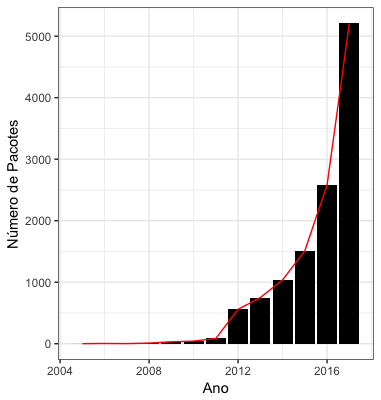
\includegraphics[width=0.8\textwidth]{./04-figuras/NRPackages}
	\fonte{\href{https://cran.r-project.org/web/packages/available_packages_by_date}
		{https://cran.r-project.org/web/packages/available\underline{ }packages\underline{ }by\underline{ }date}}
	\label{fig:RNPackages}
\end{figure}



% -----------------------------------------------------------------------------
%   Arquivo: ./02-elementos-textuais/trabalhosRelacionados.tex
% -----------------------------------------------------------------------------

\chapter{Aprendizado de máquina}
\label{chap:MachineLearning}

\section{Formulação e caracterização do aprendizado de máquina}

Nos primórdios da inteligência artificial, pesquisadores foram capazes de resolver problemas que são intelectualmente difíceis para os seres humanos, mas relativamente simples para os computadores. Exemplo disso são os problemas que podem ser descritos por uma sequência de regras ou que podem ser solucionados por operações matemáticas \cite{Goodfellow-et-al-2016}.

A dificuldade surgiu para fazer com que os computadores fossem capazes de resolver tarefas fáceis para os humanos, mas difíceis de serem descritas de forma algorítmica, como reconhecer escrita, identificar rostos em imagens ou ainda definir regras de decisão de forma autônoma \cite{Goodfellow-et-al-2016}.

Eis que surgiu o campo de Aprendizado Máquina, uma alternativa que permitia computadores aprender por exemplo e não por regras. Ao reunir o conhecimento da experiência, esta abordagem evita a necessidade de operadores humanos especificar formalmente todo o conhecimento que o computador precisa. Isso ocorre através da combinação do aprendizado de conceitos simples, em formato pré-definido, combinados de forma hierárquica para formar um aprendizado de conceitos complicados \cite{Goodfellow-et-al-2016}.

Segundo \citeonline{Cherkassky2007}, o processo de aprendizado é definido como a estimação de uma relação ou estrutura, previamente desconhecida, entre entrada e saída. Segundo o autor, o processo de aprendizado normalmente envolve três componentes \ref{fig:MLFormulation} : o \textit{Gerador} de amostras, um \textit{Sistema} que gera as saídas reais e o \textit{Aprendizado de Máquina} que estima a relação desconhecida entre entrada e saída. 

\begin{figure}[!htb]
	\centering
	\caption{Formulação do Aprendizado} 
	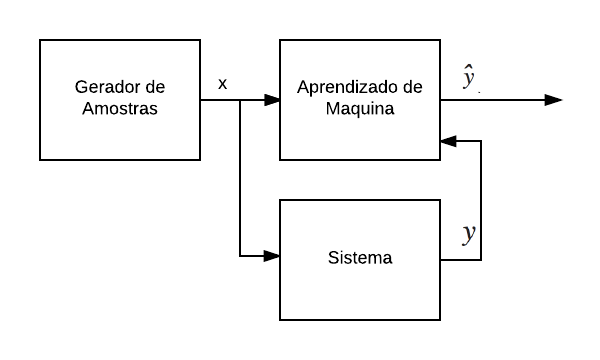
\includegraphics[width=0.8\textwidth]{./04-figuras/MLForm.png}
	\label{fig:MLFormulation}
\end{figure}

\citeonline{Cherkassky2007} explica que o \textit{Gerador} produz aleatoriamente, com distribuição de probabilidade $p(x)$, vetores $x \in {\mathbb {R}} ^{n}$, que são as características. O \textit{Sistema} é capaz de produzir, com probabilidade $p(y | x)$, saídas $y = g(x) + \epsilon$ em que $\epsilon$ é um ruido branco de $\mu = 0$. De forma geral, o \textit{Aprendizado de Máquina} é capaz de implementar uma função $\hat{y} = f(x, \omega)$, $\omega \in \Omega$, em que $\Omega$ é conjunto de parâmetros da função $f$.

O aprendizado de máquinas clássico diz respeito à aprender pelo exemplo, que é definido como um conjunto de dados, previamente obtidos pelo \textit{Gerador} e \textit{Sistema}, composto por variáveis quantitativas e qualitativas que são características do problema. Na situação onde existe uma variável resposta, o aprendizado é chamado de supervisionado, na situação onde essa variável não existe, o problema é definido como aprendizado não supervisionado. A figura \ref{fig:MLProblems} ilustra essa taxonomia, bem como algumas de suas subdivisões.


\begin{figure}[!htb]
	\centering
	\caption{Principais Problemas em Aprendizado de Máquina} 
	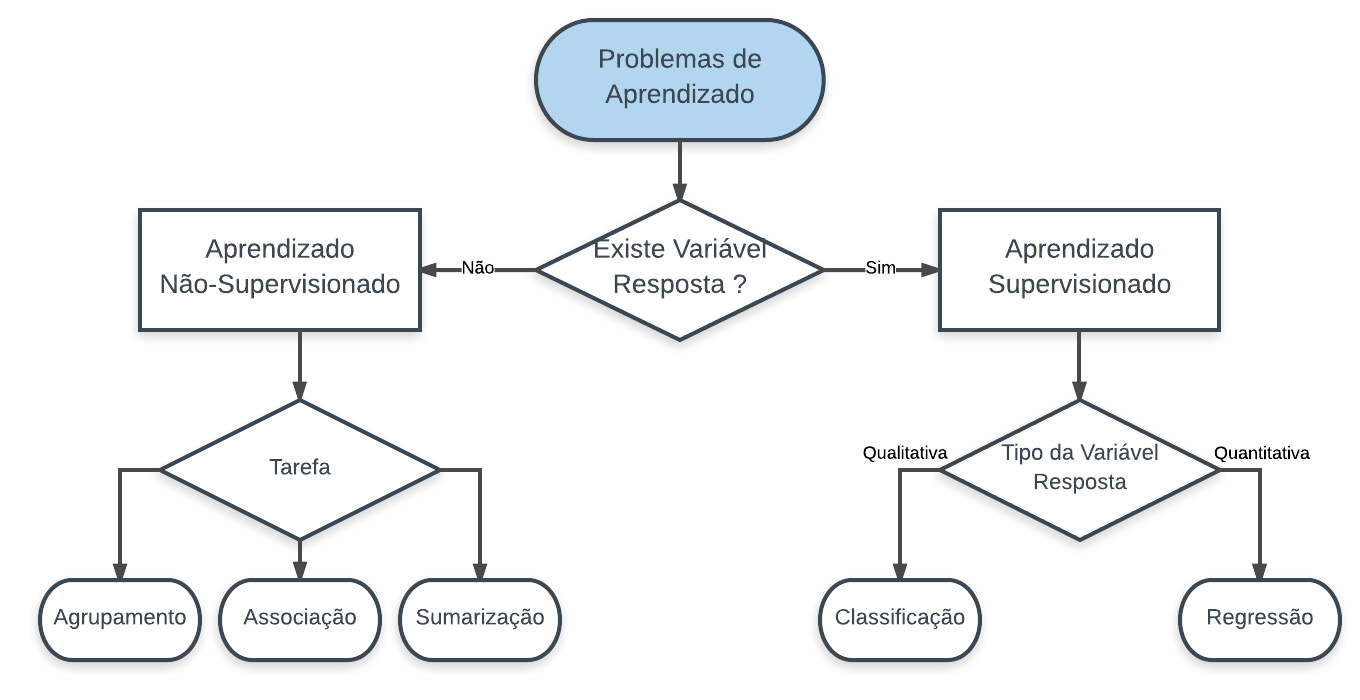
\includegraphics[width=0.8\textwidth]{./04-figuras/MLProblems.png}
	\label{fig:MLProblems}
\end{figure}
\section{Aprendizado supervisionado}

No aprendizado supervisionado, o objetivo é prever o valor de uma variável resultado com base em variáveis características. Na situação que a variável resposta é quantitativa, o problema é considerado como uma tarefa de regressão. Quando essa variável resposta é qualitativa, a tarefa é chamada de classificação.

De acordo com \citeonline{Cherkassky2007}, existem duas interpretações para o problema de aprendizado : identificação e imitação. A interpretação escolhida para fundamentar esse trabalho é a de imitação, descrita por \citeonline{Vapnik1971}.

O objetivo do aprendizado é encontrar uma função $f(x, \omega)$ que aproxima, da melhor forma possível, a saída $y$ do \textit{Sistema}. Para formular esse problema matematicamente, \citeonline{Cherkassky2007}, assumem pares de características e respostas, $(x_i, y_i)$ em que $i = (1, 2, ..., n)$ e $ n \in \mathbb {N}$, e uma função de custo $L(y, f(x, \omega))$que mede a discrepância entra saída do \textit{Sistema} $y$ e do \textit{Aprendizado de Máquina} $\hat{y}$. Então, formulam que a tarefa do aprendizado é descrita pela equação \ref{eq:LearningEq} . 

\begin{equation}
{	
	{\displaystyle {\underset {f}{\operatorname {arg\,min} }}\, L(y, f(x, \omega))}
}
\label{eq:LearningEq}
\end{equation}

A principal diferença entre problemas de classificação e regressão é a função de custo. Como a variável de saída de cada um desses problemas tem um formato diferente, a função de custo deve ser adaptada especificadamente para ele. Contudo, a formulação do aprendizado feito na equação \ref{eq:LearningEq} permanece inalterada, pois o objetivo é sempre minimizar a discrepância entre \textit{Sistema} e \textit{Aprendizado de Máquina} \cite{Cherkassky2007}.

\subsection{Problemas de classificação}
A situação mais simples de classificação é aquele em que a saída $y$ assume apenas dois valores, $y = 0$ ou $y = 1$, em que é chamada de problema de classificação binária. Nessa situação, segundo \citeonline{HastieFerro}, a função de custo específica é do formato \ref{eq:ClassProb}.

\begin{equation}
{	
	 L(y, f(x, \omega)) = \begin{dcases*}
	0,  & se $y = f(x, \omega)$ \\
	l,  & se $y \ne f(x, \omega)$ 
	\end{dcases*} \\ 
	l \in \mathbb {R^+}
}
\label{eq:ClassProb}
\end{equation}

O senário em que $y$ assume $q$ valores, em que $q > 2 \land q \in \mathbb {N}$, chamada de classificação \textit{multilabel}, pode ser simplificado em $q$ problemas de classificação binária em que o problema $j$ tem forma $y = j \rightarrow y_j = 1$ e $y_j \neq  \rightarrow y_j = 0 $, para $ 0 \leq j \leq q \land j \in \mathbb {N}$.


\subsection{Problemas de regressão}
O problema de regressão é caracterizado, segundo \citeonline{HastieFerro}, por $y \in \mathbb {R}$, dessa forma a função de custo normalmente é formulada como mostra a equação \ref{eq:RegProb}, onde $d$ é uma métrica genérica de distância entre dois números reais.

\begin{equation}
L(y, f(x, \omega)) = d(y, f(x, \omega))
\label{eq:RegProb}
\end{equation}

Nessa sistuação a variável de saída $y$ assume qualquer valor real, e a função $f$ mapeia a relação, linear ou não-linear, entre a entrada $x$ e essa saída.


\section{Métodos de Classificação} 
Nesse capítulo serão abordados os métodos de classificação implementados no pacote MLAT \cite{PauloCirinoMLAT}. 

\subsection{\textit{k Nearest Neighbours}}
O método \textit{k Nearest Neighbours} (\textbf{kNN}) é o algoritmo não paramétrico de classificação mais simples e conhecido \cite{James20131} . Seu funcionamento se dá de forma que a predição de uma amostra desconhecida é a moda das $k$ amostras mais próximas. De forma genérica sua implementação pode ser feita utilizando o pseudocódigo abaixo adaptado do trabalho de \citeonline{articleTay} :

\begin{algorithm}
	\caption{Algoritmo k-\textit{Nearest Neighbours}}
	\KwIn{$x$ amostra desconhecida,  $k$ é o parâmetro do número de vizinhos, $\{\mathbb{X}, \mathbb{Y}\}$ é o conjunto de pares amostras e respostas conhecidas }
	\KwOut{a predição da amostra desconhecida $y$ }
	
	\For {\textbf{each} $x_i \in \mathbb{X}$} {
		Computa a distância da amostra conhecida $i$ para a desconhecida $\mathbb{D_i} = d(x, x_i)$ \\
	}
	Seleciona o conjunto $\mathbb{L}$ referente as $k$ respostas com menor distância $\mathbb{D}$, onde $\mathbb{L} \in Y$ \\ 
	Computa a resposta $y = moda(\mathbb{L})$
\end{algorithm}
 

É importante ressaltar algumas características do kNN, como sua simplicidade de implementação e a não existência de uma etapa de treinamento. Além disso, o método é capaz de produzir superfícies de decisão não lineares e é robusto, dado uma escolha adequada do parâmetro $k$, a conjuntos ruidosos.

Entretanto esse algoritmo se baseia na memória das amostras conhecidas, fazendo com que ele não seja capaz de generalizar sua superfície de decisão para novas amostras fora do espaço conhecido. Outra consequência de ser um sistema baseado em memória é sua complexidade $O(n)$, para espaço e tempo, no momento de predição de cada uma das amostras de teste. 


\subsection{\textit{Support Vector Machines}}
As \textit{Support Vector Machines}, em português Máquinas de Vetor de Suporte, foram inicialmente propostas em \citeonline{boser1992training}. Esse método foi produzido como uma alternativa que, diferente de outros algoritmos tradicionais, não minimiza o erro do classificador, mas, sim maximiza a margem de separação entre duas classes \cite{James20131}. O intuito disso é produzir um classificador que seja capaz de encontrar uma superfície de decisão mais genérica, e consequentemente, que tenha melhor desempenho em amostras desconhecidas \cite{Cortes1995}.

A formulação inicial dessa metodologia sofreu adaptações e melhorias ao longo do tempo, em \citeonline{boser1992training} o classificador possuía margem rígida e assumia que existia uma superfície que separasse perfeitamente as classes, chamado hoje de \textit{Hard Margin SVM}.

Dado um conjunto de pares $(x_i, y_i)$ é possível formular esse classificador conforme a equação \ref{eq:SVMSeparavel} \cite{James20131}. Nessa formulação as respostas são $y_i \in \{1, -1\}$, $(\beta_0 + \sum_{j=1}^{p}{{\beta_i x_{ij}}})$ é o hiperplano de separação e $M$ é a variável de otimização que diz respeito ao tamanho da margem. 

\begin{equation}
\begin{split}
\underset {\beta_0, \beta_1, ..., \beta_p, M}  {\text{Maximizar : }} &{M} \\
\text{Sujeito a : } \\
&\sum_{j=1}^{p}{{\beta_j}^2} = 1, \\
&y_i(\beta_0 + \sum_{j=1}^{p}{{\beta_i x_{ij}}}) \geq M, \forall i = 1, ..., n
\end{split}
\label{eq:SVMSeparavel}
\end{equation}

Em \citeonline{Cortes1995} é demostrada uma alteração na formulação original, fazendo ser possível encontrar uma solução mesmo em problemas que as amostras não sejam completamente separáveis. Isso é feito por meio da introdução de um parâmetro $\epsilon_i$, que diz respeito a penalidade de amostras classificadas erroneamente. Essa alteração na formulação, conhecida como \textit{Soft Margin} SVM, é demonstrada pela equação \ref{eq:SVMInseparavel} \cite{James20131}.

\begin{equation}
\begin{split}
\underset {\beta_0, ..., \beta_p, \epsilon_1, ..., \epsilon_n, M}  {\text{Maximizar : }} &{M} \\
\text{Sujeito a : } \\
&\sum_{j=1}^{p}{{\beta_j}^2} = 1, \\
&y_i(\beta_0 + \sum_{j=1}^{p}{{\beta_i x_{ij}}}) \geq M(1 - \epsilon_i), \forall i = 1, ..., n, \\
&\epsilon_i \geq 0,  \sum_{i=1}^{n}{\epsilon_i} \geq C
\end{split}
\label{eq:SVMInseparavel}
\end{equation}

As equações \ref{eq:SVMSeparavel} e \ref{eq:SVMInseparavel} definem modelos de aprendizado com uma superfície de decisão linear. Para solucionar essa questão foi introduzido, em \citeonline{boser1992training} , o conceito conhecido como \textit{Kernel Trick}.

A implementação do \textit{Kernel Trick} é feita substituindo o produto interno, $f(x) = \beta_0 + \sum_{j=1}^{p}{{\beta_i x_{ij}}}$ por uma função genérica $K(x_i)$ não linear \cite{James20131}. Essa função pode introduzir termos de ordem superior ou até mesmo aplicar funções não lineares, tudo com o objetivo de facilitar a separabilidade das amostras. 
	
\subsection{\textit{Multilayer Perceptron}}
\label{sssec:MLPClassificationSubSection}
Uma rede neural artificial é formada por um conjunto de nodos, chamados de neurônios, com capacidade de processamento local e independe, agrupados em uma topologia definida \cite{Braga2007}.  O modelo \textit{Multilayer Perceptron} (MLP) é um tipo de rede neural artificial \textit{feedfoward}, que utiliza em sua camada intermediária neurônios perceptron \cite{AbadiABBCCCDDDG16}. 

\begin{equation}
y = \phi(\sum_{i = 1}^{m}{x_i  w_i} + b)
\label{eq:perceptron}
\end{equation}

O neurônio perceptron, definido pela equação \ref{eq:perceptron}, é o resultado da combinação linear dos termos das entradas $x_i$ ponderados por pesos$w_i$ e um bias $b$, após a introdução de uma não linearidade pela função de ativação $\phi$. A função de ativação $\phi$ pode assumir formatos diferentes, todavia, tradicionalmente ela é logística, tangente hiperbólica ou RELU conforme equações \ref{eq:act1}, \ref{eq:act2} e \ref{eq:act3} respectivamente \cite{Goodfellow-et-al-2016}.

\begin{equation}
\phi(z) = \frac{1}{1 + e^{-z}}
\label{eq:act1}
\end{equation}

\begin{equation}
\phi(z) = \frac{e^z - e^{-z}}{e^z + e^{-z}}
\label{eq:act2}
\end{equation}

\begin{equation}
\phi(z) = max(z, 0)
\label{eq:act3}
\end{equation}
%

A topologia da MLP, ilustrada na imagem \ref{fig:MLPDraw}, é compostas por 3 tipos de camadas : entrada, intermediária ou escondida, e, saída  \cite{Braga2007}. A rede possui uma camada de entrada com tamanho definido pelo número de variáveis do espaço dos dados de entrada. Ela pode possuir uma ou mais camadas intermediárias, formadas por neurônios perceptron, de tamanhos parametrizados por seu projetista. 

\begin{figure}[!htb]
	\centering
	\caption{Formulação do Aprendizado} 
	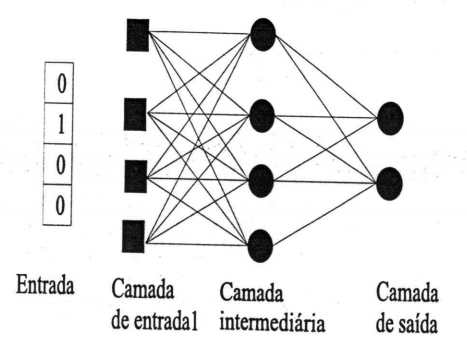
\includegraphics[width=0.8\textwidth]{./04-figuras/mlp.png} \\
	\cite{Braga2007}
	\label{fig:MLPDraw}
\end{figure}

A camada de saída em um problema de classificação, também pode assumir formatos diferentes. Para um problema binário, tradicionalmente é utilizado um neurônio do tipo logística, conforme equação \ref{eq:act1}.  No caso de problemas de classificação em que a saída pode assumir mais de 2 valores, a camada de saída deve possuir o mesmo  número de neurônios que valores de saída possíveis. Caso o projetista deseje ainda uma saída probabilística, é possível utilizar uma camada final do tipo \textit{softmax} conforme equação \ref{eq:softmax}, em que $k$ representa cada neurônio da camada de saída \cite{Goodfellow-et-al-2016}.  

\begin{equation}
\label{eq:softmax}
\sigma (\mathbf {z} )_{j}={\frac {e^{z_{j}}}{\sum _{k=1}^{K}e^{z_{k}}}}
\end{equation}

\section{Métodos de Regressão}
Nesse capítulo serão abordados os métodos de regressão implementados no pacote MLAT \cite{PauloCirinoMLAT}. 


\subsection{Regressão Linear}
O método de regressão linear é uma forma simples de performar aprendizado supervisionado, ainda assim, é um ótimo ponto de início para \textit{benchmarking} de modelos mais complicados de regressão. 

Em suma esse modelo encontra um vetor de pesos $W$ e um bias $b$ que melhor explica uma relação linear entre a entrada $x$ e a saída $y$, conforme a equação \ref{eq:LinearRegressionModel}.

\begin{equation}
\hat{y}= {x \cdot W^T} + b
\label{eq:LinearRegressionModel}
\end{equation}

Para estimar o vetor de pesos e o termo de bias é formulado um problema de otimização que minimiza a soma dos quadrados do erro residual, conforme equação  \ref{eq:LinearOpt}, utilizando o método de mínimos quadrados \cite{James20131}.

\begin{equation}
\underset {W, b}{\operatorname {arg\,min} }\ \sum_{i=1}^{n} ({y_i -  (x_i \cdot W^T+ b) })^2
\label{eq:LinearOpt}
\end{equation}

\subsection{\textit{Ridge Regression}}
\textit{Ridge Regression} é um modelo de aprendizado muito parecido com a regressão linear, a única diferença é que existe um termo adicional na função objetivo para minimizar a norma dos pesos $w_j \in W$, conforme mostra a formulação \ref{eq:LinearOptRidge} \cite{James20131} .

\begin{equation}
\underset {W, b}{\operatorname {arg\,min} }\ \sum_{i=1}^{n} ({y_i -  x_i \cdot W^T- b })^2 +  \lambda \sum_{j=1}^{m} {w_j}^2
\label{eq:LinearOptRidge}
\end{equation}

O termo $\lambda$ da equação, chamado de termo de penalização, não é otimizado pelo método, mas sim, é um parâmetro escolhido pelo projetista. Esse termo é sempre $\lambda \geq 0$, e quanto maior $\lambda$, mais os pesos referentes as variáveis não importantes são próximos de $0$ \cite{Wieringen2015}. Um caso especial desse termo é $\lambda = 0$, em que a \textit{ridge regression} se torna exatamente igual a uma regressão linear.

Dessa forma, o método de \textit{ridge regression}, têm uma tendência de generalizar melhor o aprendizado em situações em que existem muitas variáveis de entradas que não adicionam informações ao modelo \cite{Wieringen2015}.

\subsection{\textit{Multilayer Perceptron}}
Na seção \ref{sssec:MLPClassificationSubSection} foi definida a topologia da rede neural artificial MLP para o problema de classificação, entretanto, esse método também pode ser utilizado para problemas de regressão.

Nessa situação as camadas de entrada e intermediária permanecem exatamente iguais, a única mudança necessária é na camada de saída. Para regressão a camada de saída é um único neurônio linear conforme mostrado pela equação \ref{eq:neuronLinear} \cite{Goodfellow-et-al-2016}.  

\begin{equation}
\phi(z) = z
\label{eq:neuronLinear}
\end{equation}

	
% -----------------------------------------------------------------------------
%   Arquivo: ./02-elementos-textuais/trabalhosRelacionados.tex
% -----------------------------------------------------------------------------



\chapter{Estatísticas de teste}
\label{chap:testStatistics}

\section{Definição de estatística de teste}
Uma estatística de teste é o valor que é calculado a partir de dados durante um teste de hipóteses. O valor dessa estatística mede o grau de concordância entre uma amostra de dado e a hipótese nula, que por sua vez pode ser rejeitada ou não \cite{Casella2002}. 

Em um teste estatístico, as hipóteses são premissas a serem testadas. Tradicionalmente existem duas hipóteses, a nula e a alternativa, em que o objetivo do teste é conservadoramente rejeitar a hipótese nula à favor da hipótese alternativa. Dessa forma, os testes são feitos tal que o objetivo que deseja-se testar é descrito pela hipótese alternativa.

\section{Testes paramétrico e não-paramétrico}
Um teste estatístico paramétrico é aquele que faz suposições sobre os parâmetros da distribuição geradora das populações que estão sendo testadas. Desta forma, um teste não-paramétrico é aquele que implica a ausência dessas suposições, de forma mais direta é aquele que não supões nada sobre os parâmetros da função de distribuição de probabilidade geradora \cite{LowryTrem}.

Na maioria das situações práticas, os teste não-paramétricos são vantajosos quando as populações de teste são muito pequenas, possuem estrutura ordinal, ou são melhor representadas pela mediana. Quase que em todas as demais situações, os testes paramétricos se comportam de forma mais confiável e geram resultados com maior potência estatística \cite{Casella2002}.

Além disso, os teste paramétricos não estão limitados pela suposição de que a dispersão amostral é igual nas populações de teste, diferente da maioria dos não-paramétricos, e tampouco funciona apenas para funções geradoras normais. Dado um tamanho amostral suficientemente grande, qualquer distribuição pode ser aplicado para um teste que assume
normalidade \cite{KernsFerro}.

\subsection{ANOVA}
%O teste estatístico análise de variância, comumente conhecido como ANOVA, permite avaliar a existência de diferença significativa entre médias de populações diferentes, e se os fatores exercem influência em alguma variável dependente \cite{milone2004estatística}. Nesse teste, a hipótese nula é que as médias populacionais são iguais e a hipótese alternativa é que pleo menos uma é diferente. Além disso, o ANOVA, é chamado de paramétrico pois assume que as amostras são aleatórias e independetes, que as populações seguem distribuição normal e possuem variância iguais.

No caso do teste entre classificadores em bases de dados diferentes, o ANOVA divide a varabilidade total entre variabilidade entre algoritmos, bases de dados e erro residual. Se a variabilidade entre algoritmos é significantemente maior que a variabilidade do erro, é possível rejeitar a hipótese nula afavor da hipótese alteranativa \cite{demvsar2006statistical}.

O resultado do teste ANOVA permite afirmar se todos o algoritmos perforam igualmente ou não, é importante notar que ele não diz respeito qual é melhor ou pior que os demais. Para auxiliar com essa informação exitem dois testes que podem ser aplicados aposteriori, teste de Tukey e teste de Dunnett. Para comparar todos os métodos entre sí é necessário a utilização do teste de Tukey, o teste de Dunnet por outro lado compara todos os métodos com um base \cite{demvsar2006statistical}.

\subsection{Friedman}

O teste de Firedman é um equivalente não paramétrico ao teste ANOVA, em que seu resultado é um rank da performace de todos os métodos. A hipóse nula desse teste é que a diferença entre os pares segue uma distribuição simétrica em torno de 0, e a hipótese alternativa é que não segue essa distribuição \cite{Casella2002}.

É importante notar que a principal vantagem do teste de Friendman, quando comparado ao teste ANOVA, é que ele não assume premissas quanto a distribuição dos resultados, e mais importe ainda é que ele não assume que as variâncias são iguais. Isso é importante porque não nescessariamente os resultados assumem distribuições normais, e tampouco os eles possuem mesma variância para bases diferentes \cite{demvsar2006statistical}. Por último, o rank do teste de Firedman remove a necessidade da realização de testes a posteriori para comparar quais métodos são melhores que os demais.








% -----------------------------------------------------------------------------
%   Arquivo: ./02-elementos-textuais/trabalhosRelacionados.tex
% -----------------------------------------------------------------------------



\chapter{O pacote MLAT }
\label{chap:TheSoftware}
A tarefa de criação de um novo modelo de aprendizado de máquina passa por algumas etapas bem definidas, como, implementação, \textit{benchmarking} e análise de resultados, conforme mostra o diagrama da figura \ref{fig:BuildingMLModel}.

\begin{figure}[!htb]
	\centering
	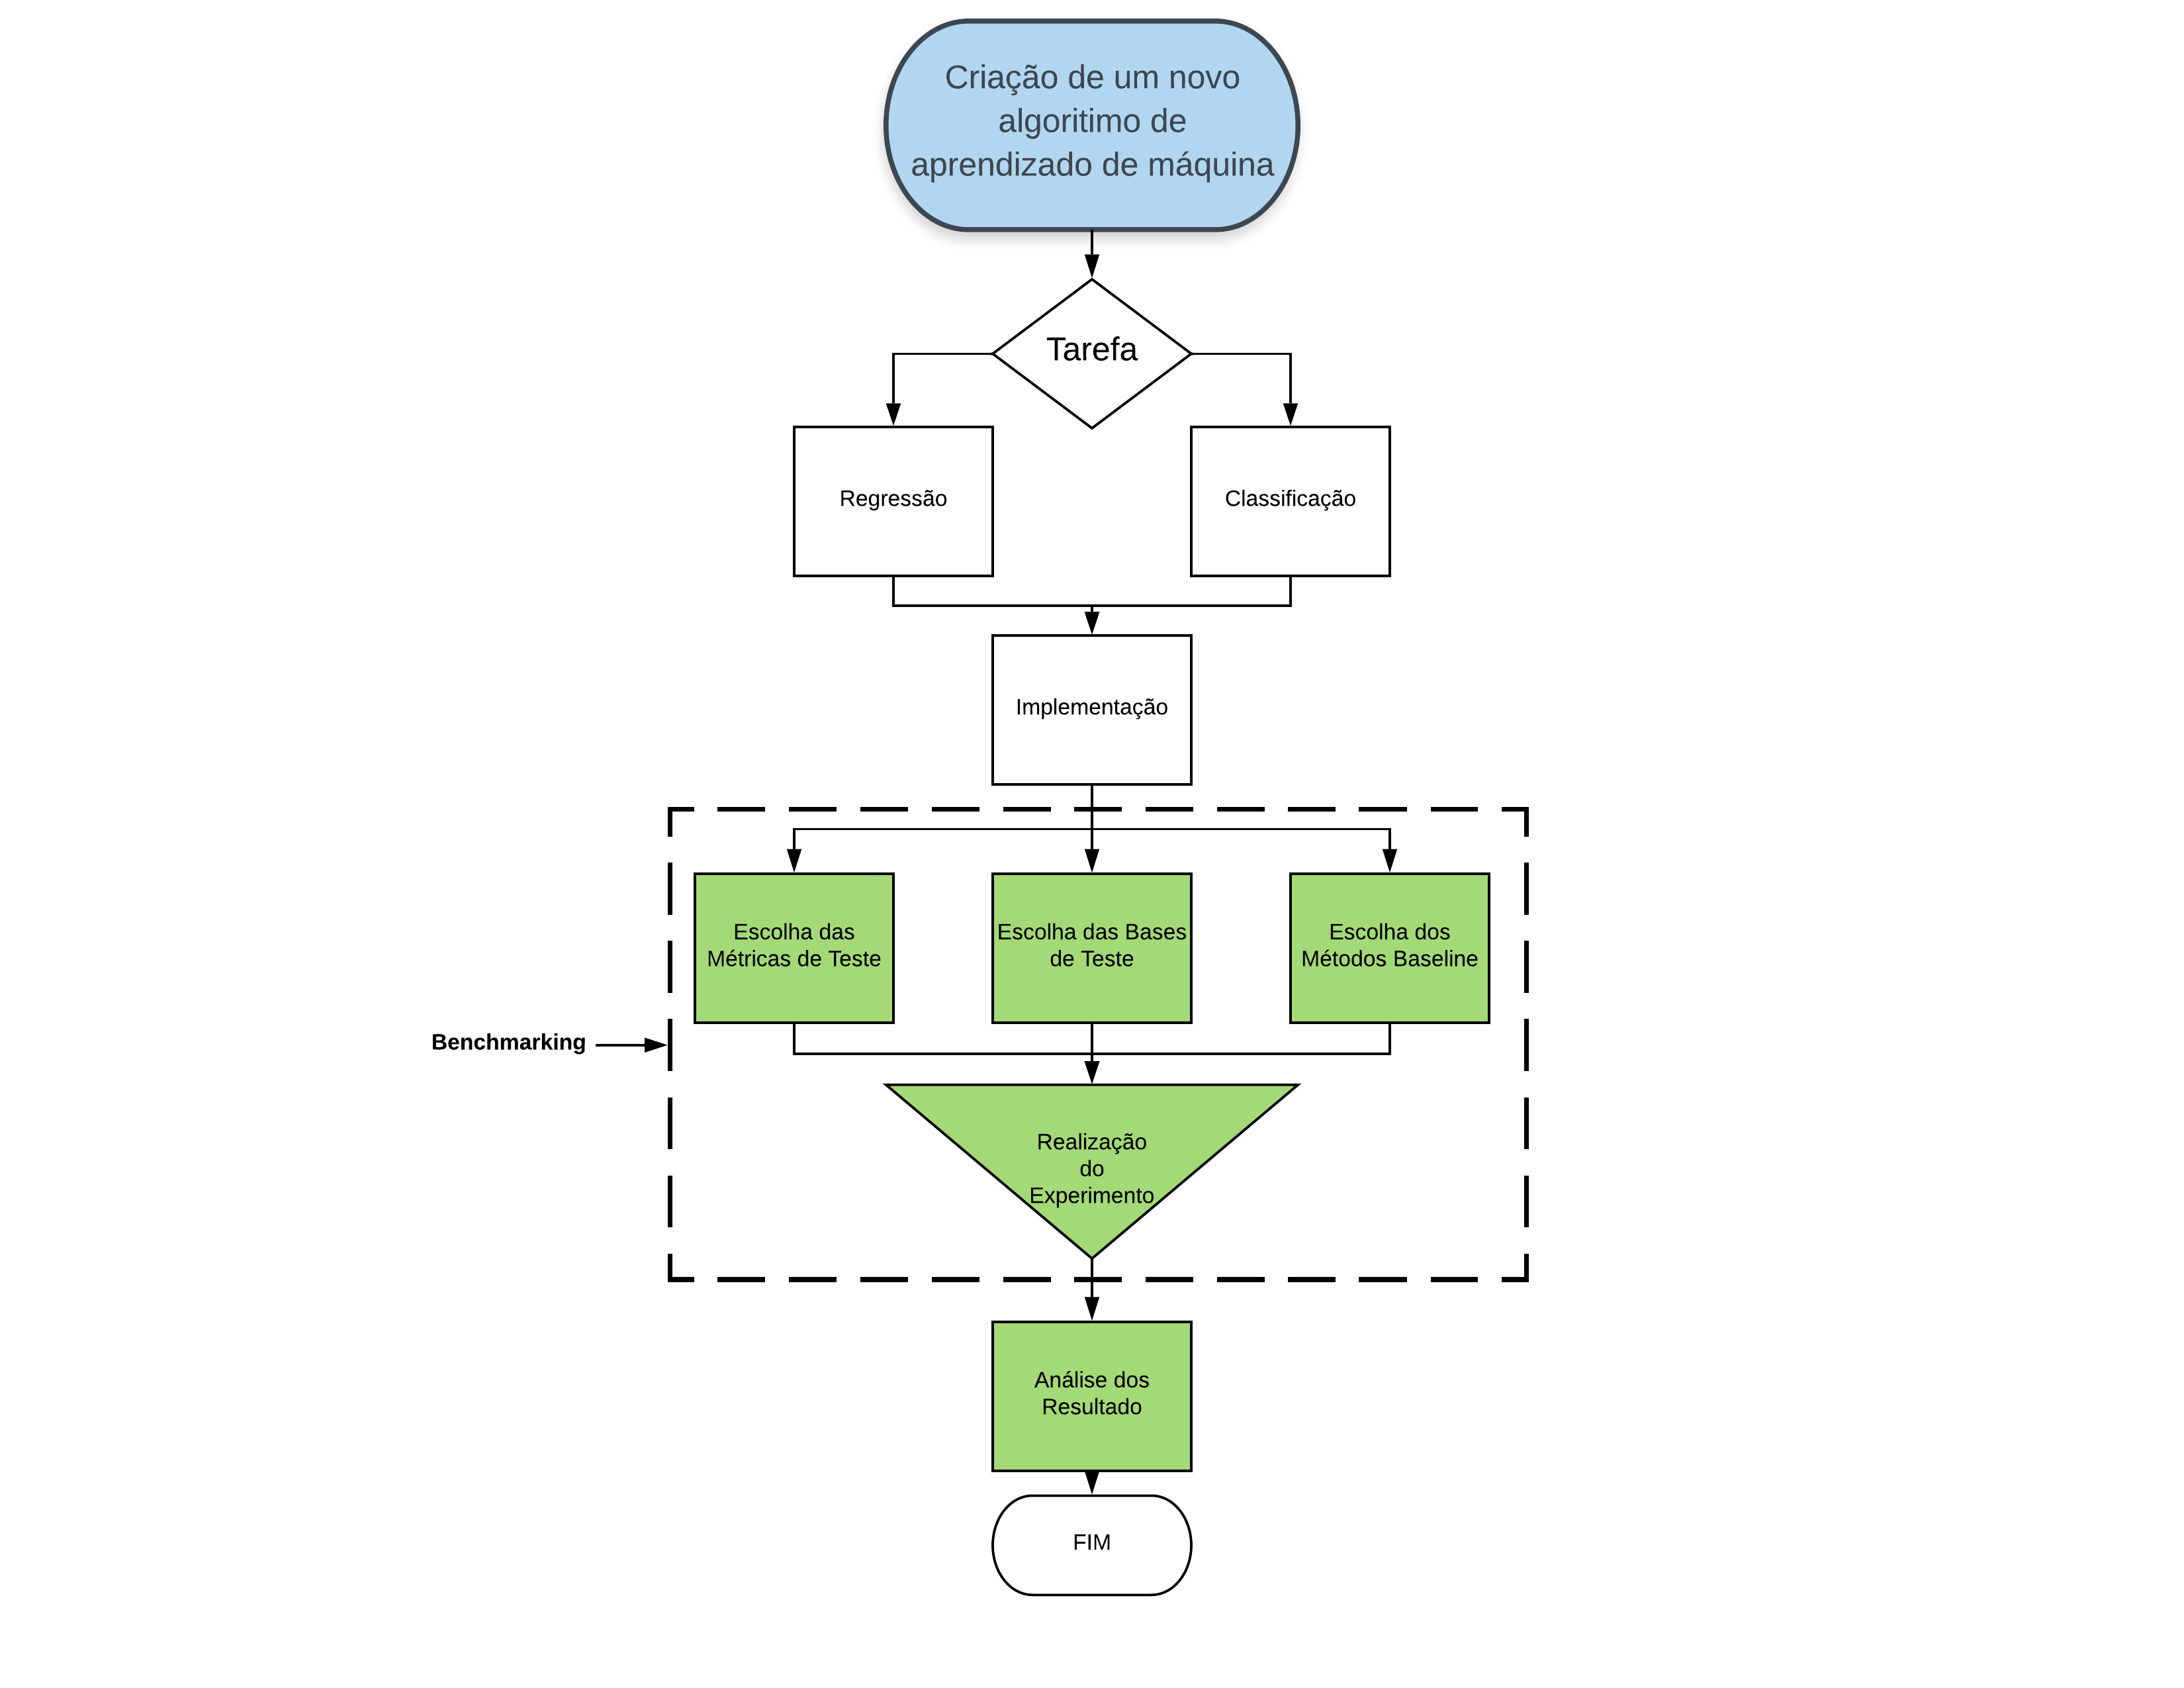
\includegraphics[width=\textwidth]{./04-figuras/BuildingNewMethod.png}
	\caption{Etapas da construção de um novo modelo de aprendizado.} 
	\label{fig:BuildingMLModel}
\end{figure}

O pacote \textit{Machine Learning Atutomated Testing} (MLAT) têm como objetivo automatizar e simplificar algumas dessas etapas, representadas de verde no diagrama da figura \ref{fig:BuildingMLModel}. 

Nesse capítulo será descrito cada uma dessas etapas e como, o pacote MLAT, vai auxiliar seus usuários em cada uma delas. Por fim, será apresentado a forma de utilização do pacote e uma implementação exemplo.

\section{Métodos Baseline}
\label{sec:Metodos}
Os métodos baseline foram divididos em três grupos : regressão, classificação binário ou \textit{multylabel}. Foi importante dividir os métodos nesses três grupos porque o mesmo foi feito para as bases de dados e métricas de teste. Essa decisão de projeto possibilitou uma simplicidade na interface do usuário, em que ele apenas informa o programa a tarefa e é possível obter todos os métodos, bases e métricas que serão possíveis de serem utilizadas.

No MLAT foram implementados, inicialmente, os métodos descritos no capítulo \ref{chap:MachineLearning} para as três tarefas citadas acima. O pacote fornece uma interface que o usuário pode apenas informar a tarefa e o programa retorna uma lista com os métodos e suas parametrizações padrão, ou ainda, o usuário pode criar uma lista com os métodos e suas próprias parametrizações. 

\section{Métricas de Testes}
\label{sec:Metricas}
Todo algorítimo de aprendizado de máquina, implicitamente ou explicitamente, tem como objetivo minimizar algum tipo de erro. Todavia, o erro minimizado, pode ser diferente entre os modelos, ou ainda, não representar o verdadeiro objetivo do aprendizado. Dessa maneira, durante a comparação entre os modelos de aprendizado, é importante definir a priori métricas representatívas do verdadeiro objetivo do aprendizado, para ser possível comparar os modelos da maneira justa.

Para fazer isso, o pacote MLAT, permite ao usuário escolher entre mais de 20 possíveis métricas de avaliação divididas em três tarefas. Para utilizar qualquer uma das métricas, o usuário, precisa informar ao pacote os nomes das métricas desejadas ou escolher entre as tarefas de regressão, classificação binária ou \textit{multylabel}.

\section{Bases de Teste}
\label{sec:Bases}
Algumas bases de dados, como MNIST \cite{lecun} ou \textit{Spam or Ham} \cite{zezim}, se tornaram problemas clássicos para se comparar o desempenho de novos modelos de aprendizado de máquina. Com o objetivo de poupar o usuário da busca e preparo das bases de dados clássicas, foi implementado no pacote uma forma de carregamento em que ele apenas informa os nomes das bases ou a tarefa de aprendizado. Após a escolha das bases o pacote aplica os modelos em cada uma das bases de maneira autônoma, informando o usuário apenas as métricas de testes.

É importante salientar, que nessa versão do pacote, é possível serem utilizadas apenas as bases de disponibilizadas. Essa foi uma decisão de projeto que garantiu um funcionamento mais otimizado do pacote e que possibilitou uma interface mais simples para o usuário. 

Até o momento foram disponibilizadas 20 bases, e na próxima versão do MLAT, haverá uma interface que possibilitará a adição de qualquer base por meio de uma função que à colocará no padrão do pacote.

\section{Realização do Experimento}
A realização do experimento culmina na combinação das três etapas anteriores, descritas nas seções \ref{sec:Metodos}, \ref{sec:Metricas} e \ref{sec:Bases}. Nesse momento o usuário pode informar ao programa alguns parâmetros do teste, como o percentual do \textit{split} entre treino e teste, e o número de vezes que cada teste será realizado para os pares de algoritmo e parametrização. Ao fim do processo é entregue ao usuário uma tabela que contêm todos as métricas dos resultados de cada iteração de teste.

\section{Análise dos  Resultados}
A etapa de análise dos resultados é o momento em que o projetista deve escolher uma métrica objetivo para que ele possa comparar os diferentes métodos treinados. A saida desse momento deve ser capaz de auxiliar o projista no julgamento de qual método tever melhor desempenho no experimento. Para cumprir esse objetivo, o pacote permite ao usuário escolher e performar um dos testes estatísticos descritos no capítulo \ref{chap:testStatistics}. 



\section{Uso do MLAT}

\begin{figure}[!htb]
	\centering
	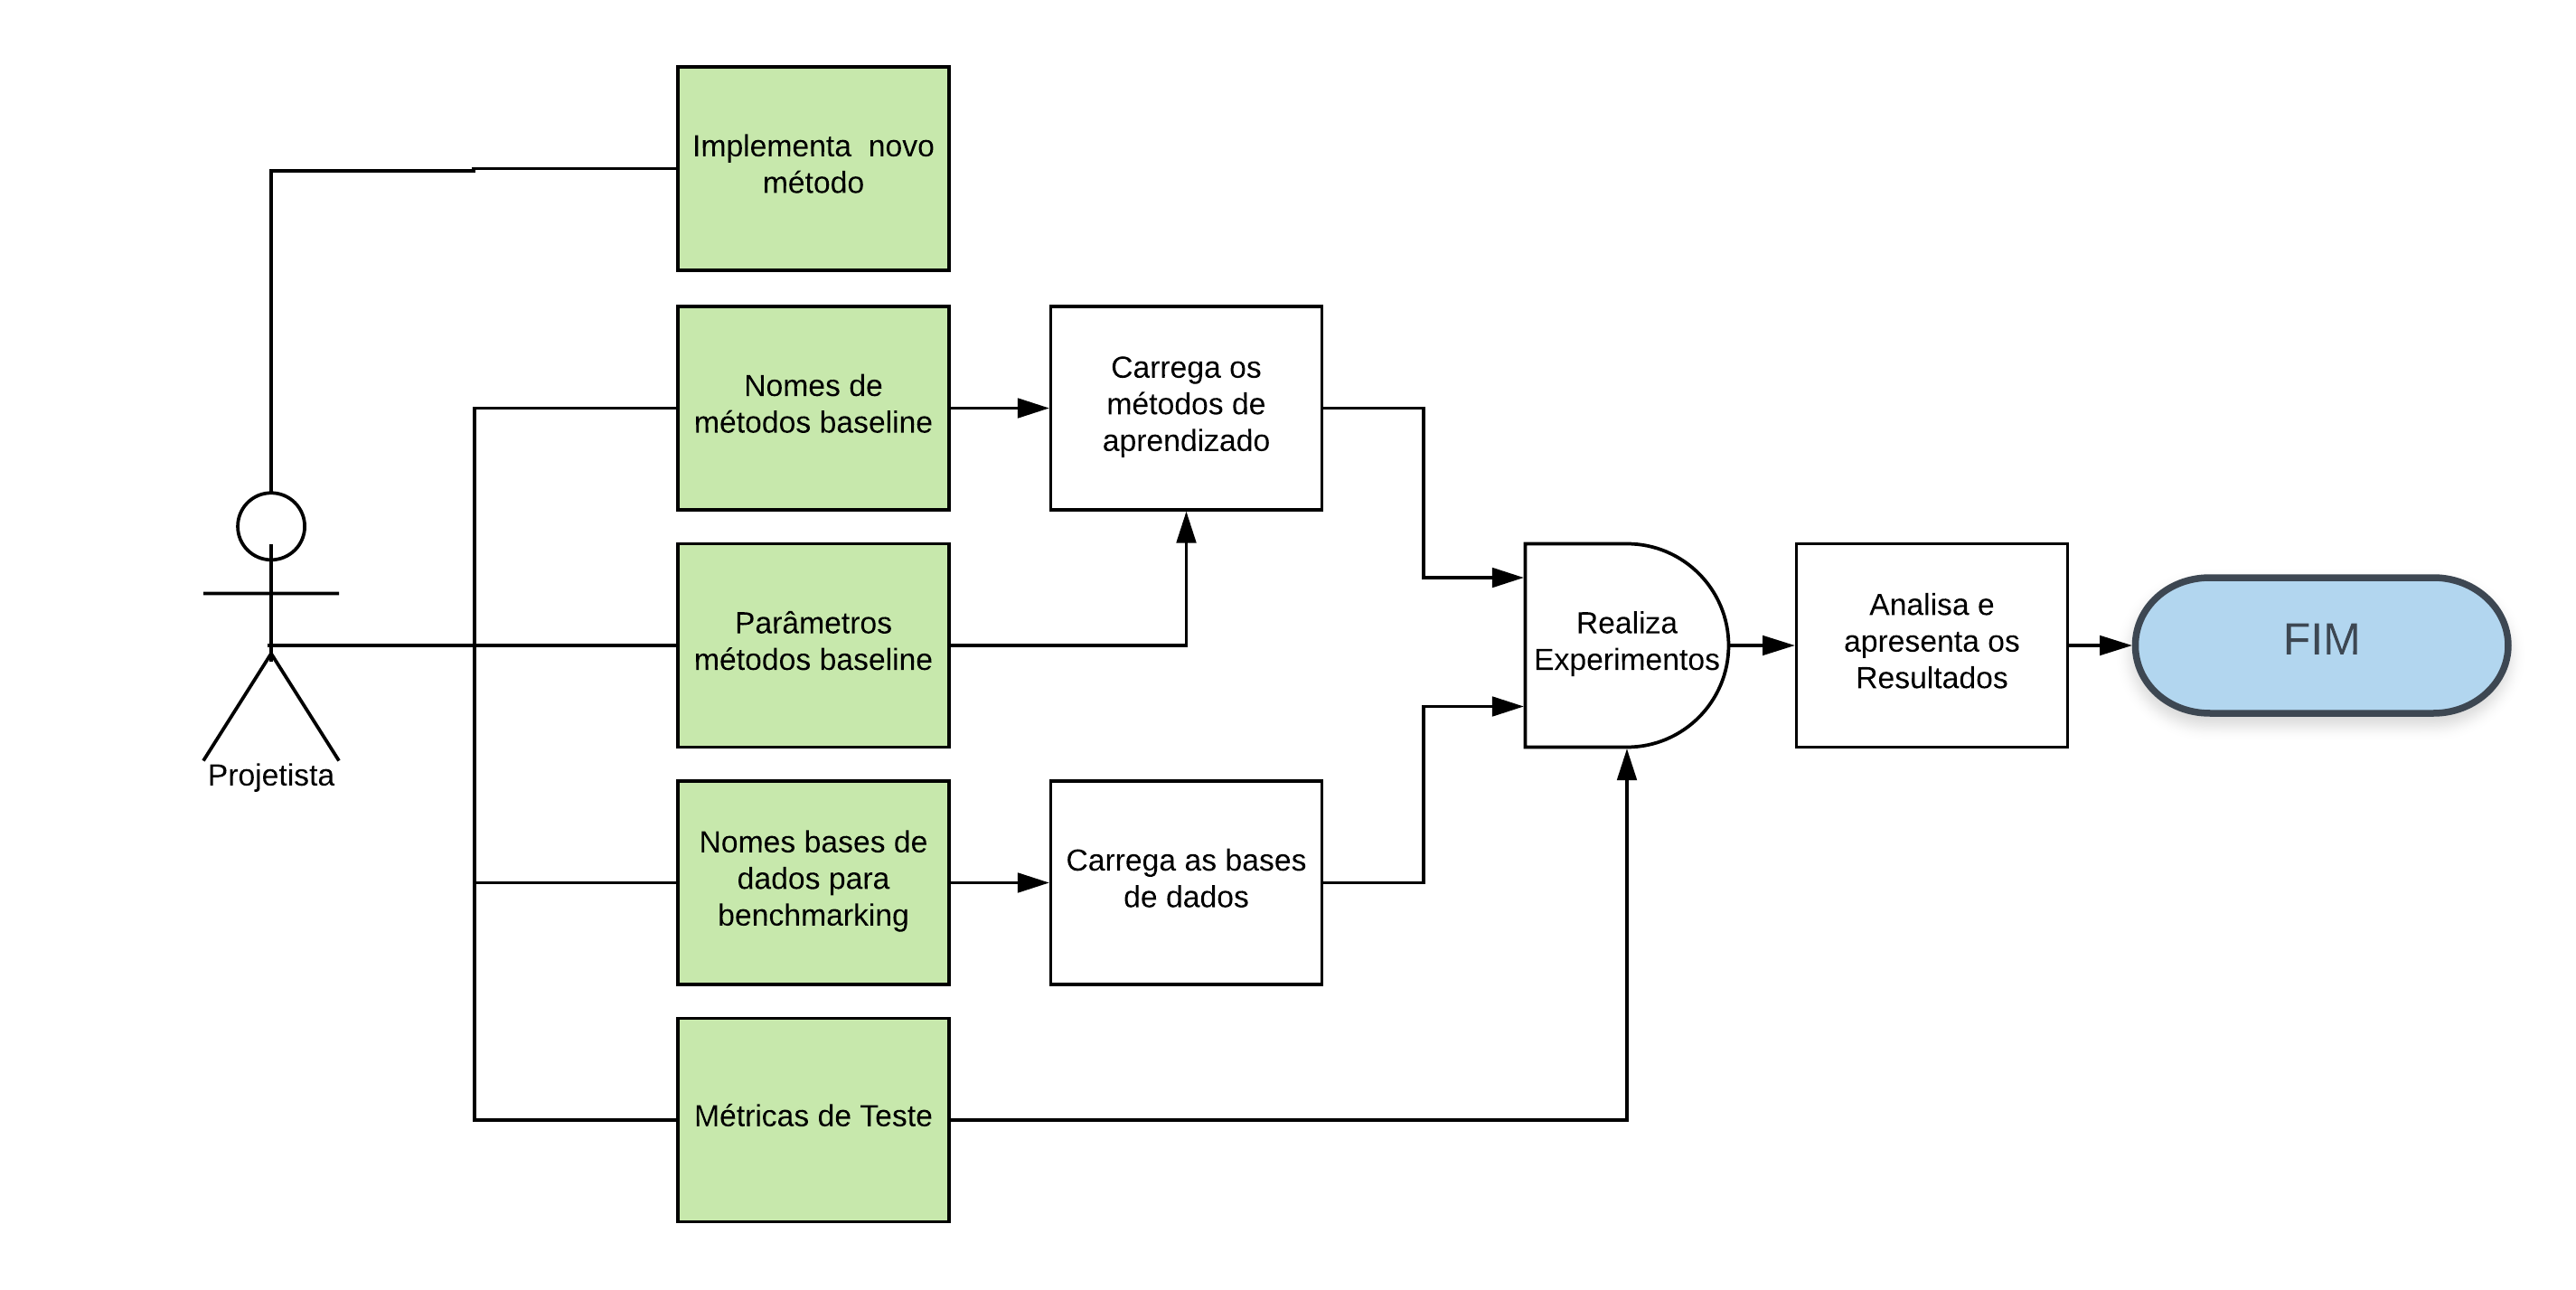
\includegraphics[width=\textwidth]{./04-figuras/UseCase.png}
	\caption{Utilização do Pacote MLAT.} 
	\label{fig:BuildingMLModel}
\end{figure}


\begin{lstlisting}[language=R]

### Carrega e instala pacotes
install.packages('devtools')
require('devtools')
devtools::install_github('PauloCirino/MLAT')
require('MLAT')

### O novo algoritmo
MyNewAlgoFunc <- function(X_train, Y_train, X_test, k) {
Y_hat <- numeric()
for( i in 1:nrow(X_test)){
x_iter <- X_test[i, ]
distVet <- apply(X_train, 1, function(x){
sum( abs(x_iter - x ) )
})
Y_iter_vet <- Y_train[ order(distVet) ] [1:k]
Y_iter_aux <- numeric()
for(j in 1:k){
Y_iter_aux <- append(Y_iter_aux,
rep(Y_iter_vet[j],
k - j + 1) )
}
unique_y <- unique(Y_iter_aux)
aux_Table <- tabulate(match(Y_iter_aux,  unique_y))
Y_hat[i] <- unique_y[which.max(aux_Table)]
}
Y_hat
}

### Parametriza teste
task <- 'MultClass'
cmpTestsFuncsList <- MLAT::GetAllMultClassAlgo()
dataSetNames <- MLAT::GetDataSetsNames(task = task)
testMetrics <- MLAT::GetMetrics(task = task)

### Coloca minha funcao no padrao do pacote
newAlgoInStandarts <- MLAT::CreateAlgo(  
algoName = 'KNN Mahalanobis Ponderado', 
algoFun = MyNewAlgoFunc, 
task = task, 
paramList = list(k = 2:10) )
cmpTestsFuncsList[[length(cmpTestsFuncsList) + 1]] <- newAlgoInStandarts

### Realiza experimento
myResult <- RunTests( cmpTestsFuncsList = cmpTestsFuncsList,
task = task,
dataSetNames = dataSetNames,
metrics = testMetrics,
nTestsPerParam = 10,
splitPerc = 0.7, 
verbose = TRUE)

\end{lstlisting}



%   Insere os elementos pós-textuais
\postextual
% -----------------------------------------------------------------------------
%   Arquivo: ./03-elementos-pos-textuais/referencias.tex
% -----------------------------------------------------------------------------



% -----------------------------------------------------------------------------
%   Carrega o arquivo “myRefs.bib” e extrai automaticamente as referências citadas
% -----------------------------------------------------------------------------

\bibliography{./03-elementos-pos-textuais/myRefs}{}
\bibliographystyle{abntex2-alf}		% Define o estilo ABNT para formatar a lista de referências  


% -----------------------------------------------------------------------------
%   Este arquivo não necessita de ser editado.
% -----------------------------------------------------------------------------
		% Referências
%\include{./03-elementos-pos-textuais/glossario}		% Glossário
%% -----------------------------------------------------------------------------
%   Arquivo: ./03-elementos-pos-textuais/apendices.tex
% -----------------------------------------------------------------------------



\begin{apendicesenv}
\partapendices



% -----------------------------------------------------------------------------
% Primeiro apêndice
% -----------------------------------------------------------------------------


\chapter{Manual do pacote MLAT} 			% edite para alterar o título deste apêndice
\label{chap:apendiceManual}
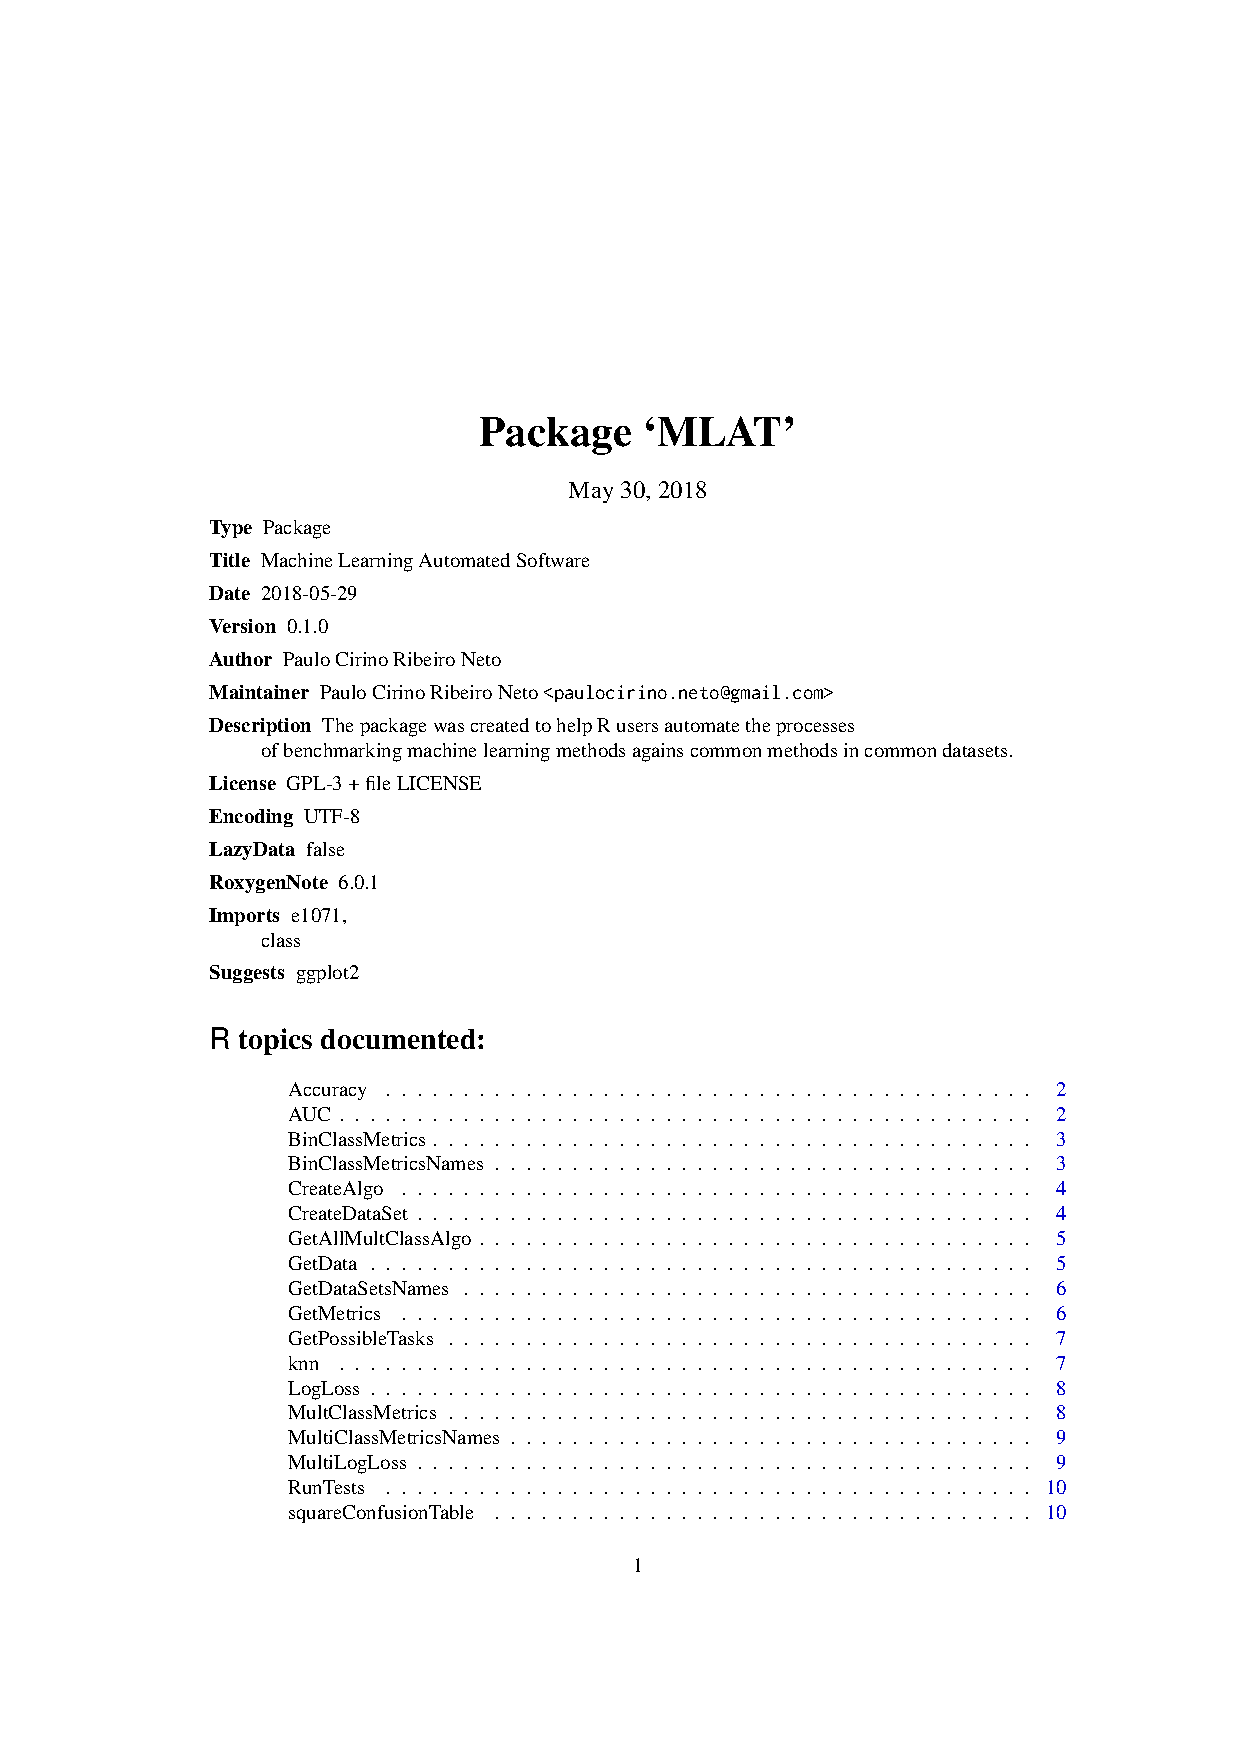
\includepdf[pages=-,pagecommand={},width=\textwidth]{manual.pdf}


\end{apendicesenv}

			% Apêndices
%% -----------------------------------------------------------------------------
%   Arquivo: ./03-elementos-pos-textuais/anexos.tex
% -----------------------------------------------------------------------------



\begin{anexosenv}
\partanexos



% -----------------------------------------------------------------------------
% Primeiro anexo
% -----------------------------------------------------------------------------

\chapter{Nome do anexo}		% edite para alterar o título deste anexo
\label{chap:anexoA}

Lembre-se que a diferença entre apêndice e anexo diz respeito à autoria do texto e/ou material ali colocado.

Caso o material ou texto suplementar ou complementar seja de sua autoria, então ele deverá ser colocado como um apêndice. Porém, caso a autoria seja de terceiros, então o material ou texto deverá ser colocado como anexo.

Caso seja conveniente, podem ser criados outros anexos para o seu trabalho acadêmico. Basta recortar e colar este trecho neste mesmo documento. Lembre-se de alterar o "label"{} do anexo.

Organize seus anexos de modo a que, em cada um deles, haja um único tipo de conteúdo. Isso facilita a leitura e compreensão para o leitor do trabalho. É para ele que você escreve.


% -----------------------------------------------------------------------------
% Novo anexo
% -----------------------------------------------------------------------------

\chapter{Dica: nomes no BibTeX}
\label{chap:anexoB}

Reproduzo neste anexo, \textit{ipsis litteris}, o texto de autoria de \citeonline{Queiroz2014}.

Se você utiliza LaTeX para a redação de artigos já deve ter se deparado com algum tipo de problema no modo como o nome dos autores é apresentado no documento final (pior é quando a "descoberta"{} ocorre depois de já ter submetido o paper). Muitas vezes é difícil encontrar uma maneira certa de escrever o nome no arquivo *.bib e garantir que ele seja transcrito corretamente independente do estilo utilizado. Este texto tem o intuito de discutir o modo como o BibTeX interpreta o nome dos autores e ajudar na árdua tarefa de organizar a bibliografia.

Pessoalmente eu prefiro fornecer o nome completo dos meus autores para o BibTeX, sem abreviações e sem omitir nomes, quando possível. Desse modo, eu dou garantia que a minha bibliografia irá conter todos os dados para referenciar o autor independente do estilo utilizado para apresentá-lo. Depois disso, eu simplesmente espero que o BibTeX faça a abreviação e a colocação dos nomes da maneira correta de acordo com o estilo indicado. No entanto, para que essa tarefa seja feita é preciso apresentar os nomes da maneira correta para que a sua divisão seja feita de forma apropriada.

Para entender como o BibTeX divide um nome, é preciso conhecer antes as diversas partes que podem compor o nome de uma pessoa, que, a princípio, são: primeiro nome, nome do meio, ligação, último nome e júnior. A descrição de cada uma dessas partes é feita a seguir.

\begin{compactitem}
	\item \textbf{Primeiro nome:} é o nome da pessoa, geralmente utilizado para identificar uma pessoa em um contexto informal. Ex.: Diego, João, Maria etc. Em alguns casos o primeiro nome pode ser composto por dois nomes, como Maria Ana, Victor Hugo, etc. Nestes casos, deve-se observar como a pessoa utiliza o nome para poder diferenciar a segunda parte como Primeiro nome ou Nome do meio.

	\item \textbf{Nome do meio:} é o nome que sucede o primeiro nome, mas antecede o último nome, geralmente abreviado, por simplicidade. Ex.: Alan Mathison Turing, "Mathison"{} é o nome do meio. É comum uma pessoa possuir mais do que um nome do meio e também é comum que o nome do meio de alguns autores seja desconhecido, devido às abreviações e omissões feitas pelo mesmo.

	\item \textbf{Ligação:} também chamado de separador, são as palavras "de"{}, "da"{}, "do"{}, "e"{}, "von"{}, entre outras que ligam um nome ao outro. Em John von Neumann e Ricardo Luis de Azevedo da Rocha, por exemplo, as palavras "von"{}, "de"{}  e "da"{}  são as ligações. Num contexto geral, elas normalmente são grafadas com inicial minúscula para não serem confundidas com o nome do meio e, embora não seja comum em todos lugares do mundo, no Brasil é comum um nome possuir até mais do que uma ligação.

	\item \textbf{Último nome:} também chamado de nome de família, é o nome utilizado para identificar uma pessoa em situações formais, como referência em artigos, livros etc. Ex.: Albert Einstein, "Einstein"{} é o último nome.

\item \textbf{Júnior:} é um sufixo do nome que indica a existência de um parente com o mesmo nome. Geralmente abreviado como "Jr."{} pode ser apresentado de diversas formas como "Filho"{}, "Neto"{} ou traduzido para o idioma de origem do dono do nome, como "fils"{} (filho) em francês. Ex.: John Forbes Nash Jr.
\end{compactitem}

Quando indicamos o nome de um autor no BibTeX ele interpreta os nomes seguindo uma das três regras a seguir:

\begin{compactenum}
	\item \textbf{Nenhuma vírgula:} {Primeiro nome} {ligação} {Último nome}

	\item \textbf{Uma vírgula:} {ligação} {Último nome}, {Primeiro nome}

	\item \textbf{Duas vírgulas:} {ligação} {Último nome}, {Júnior}, {Primeiro nome}
\end{compactenum}

Como pode-se notar, a distinção entre essas três possíveis interpretações se dá com base na quantidade de vírgulas que foram inseridas e no posicionamento da ligação, que devem sempre ser escritas com a inicial minúscula. O(s) nome(s) do meio são todos os nomes que estão após o primeiro nome, porém antes da ligação e do último nome. A princípio, o BibTeX interpreta os nomes do meio como sendo parte do primeiro nome.

Para mostrar como isso pode gerar problemas, imagine, por exemplo, se o nome "John Forbes Nash Jr."{} fosse apresentado em um arquivo BibTeX. Como nenhuma vírgula foi inserida, será entendido que "John Forbes Nash"{} é o primeiro nome e "Jr."{} é o último nome, o que não seria correto. De forma semelhante, se for apresentado na forma "Nash Jr., John Forbes", então "John Forbes"{} será o primeiro nome enquanto "Nash Jr."{} será o último nome, que também está incorreto.

Portanto, a maneira correta de referenciar seria utilizando a terceira opção pois é a única que inclui o Jr. (utilizando duas vírgulas): "Nash, Jr., John Forbes"{}, fazendo com que "John Forbes"{} seja compreendido como primeiro nome, "Nash"{} como último nome e "Jr."{} como o júnior.

Outro grande problema ocorre quando um nome possui mais do que uma ligação, como em "Ricardo Luis de Azevedo da Rocha"{}. Quando o BibTeX lê um nome como esse, ele entende que tudo que vem após o ligador, faz parte do último nome. Neste caso, "Ricardo Luis"{} seria tratado como o primeiro nome e "Azevedo da Rocha"{} como último nome.

Para evitar esse comportamento, devemos optar pela segunda opção (utilizando uma vírgula), ou seja, "da Rocha, Ricardo {Luis de} Azevedo"{}, fazendo com que o último nome seja somente "Rocha"{} e precedido pelo seu ligador.

Note que neste último exemplo o ligador e o nome que o antecede foram delimitados por chaves. Este é um pequeno e útil truque que pode ser feito para garantir que os ligadores não sejam inclusos ao abreviar nomes (Ex.: Universidade de São Paulo, abrevia-se U.S.P. ao invés de U. de S.P. ou U.d.S.P.). Fazendo isso, o BibTeX passa a tratar "Luis de"{} como um único nome e o abrevia corretamente quando necessário.

E qual a importância de garantir que o BibTeX interprete corretamente as diversas partes de um nome? A verdade é que cada estilo trata o nome de uma maneira diferente: o IEEE, por exemplo, coloca apenas as iniciais do primeiro nome e a ligação seguida do último nome; a Nature, por outro lado, coloca a ligação e o último nome, seguido das iniciais do primeiro nome; e assim por diante. Assim sendo, entender como os nomes são interpretados nos ajuda a garantir que o mesmo seja sempre dividido da maneira correta e formatado apropriadamente independente do estilo fornecido.

Por fim, e não menos importante, também deixo aqui um aviso sobre a acentuação no BibTeX. Eu já presenciei diversos problemas com relação a acentuação nos nomes dos autores, títulos dos artigos etc. Em especial os problemas ocorreram quando eu estava utilizando o abnTeX, que é um projeto que tem o objetivo de implementar o padrão ABNT em formato TeX. Embora este projeto não seja um dos mais ativos, ele ainda é muito utilizado e alguns grupos de pesquisa utilizam estilos que nada mais são do que versões derivadas deste (como é o caso do laboratório que faço parte).

O problema é que este estilo possui uma falha (descrita em \href{http://abntex.codigolivre.org.br/node5.html}{http://abntex.codigolivre.org.br}), que impede que acentos sejam convertidos corretamente em letras maiúsculas. Para contornar o problema eles pedem que sejam utilizados códigos para descrever os acentos nos arquivos *.bib ao invés de inserí-los diretamente pelo teclado. Dado a quantidade de problemas que essa falha me gerou, julgo isso como uma boa prática e deixo aqui a minha recomendação de que não sejam utilizados caracteres não-ASCII nos arquivos *.bib.

Como os arquivos *.bib são interpretados pelo LaTeX, é possível utilizar alguns comandos em seus campos. A saber, segue os comandos para formar os acentos mais comuns:
\\
\\
\\



[A parte final do texto original foi suprimida, por conter incorreções.]\footnote{Nesta parte era apresentado os comandos \LaTeX{} para acentuação. No entanto, foi constatado que os comandos, se utilizados como apresentado, provocariam erros na transformação de  minúsculas para maiúsculas e vice-versa, algo bastante recorrente no estilo \texttt{abntex2}. Para a tabela com os comandos corretos veja \autoref{fig:acentosLatex}.}.
\\
\\
\\

[Em \href{http://en.wikibooks.org/wiki/LaTeX/Special_Characters}{http://en.wikibooks.org/wiki/LaTeX/Special\underline{ }Characters}] você encontra diversos outros acentos e símbolos para serem utilizados no LaTeX.


Referência:\\

Alexander Binder. Help On BibTeX Names. Disponível em <\href{www.kfunigraz.ac.at/~binder/texhelp/bibtx-23.html}{www.kfunigraz.ac.at/...}>. Acessado em 4 de março de 2011.




\end{anexosenv}			% Anexos
%% -----------------------------------------------------------------------------
%   Arquivo: ./03-elementos-pos-textuais/indiceRemissivo.tex
% -----------------------------------------------------------------------------



% -----------------------------------------------------------------------------
%   Este comando gera automaticamente o índice remissivo para os termos definidos
%   no corpo do documento
% -----------------------------------------------------------------------------

\printindex	 


% -----------------------------------------------------------------------------
%   Este arquivo não necessita de ser editado.
% -----------------------------------------------------------------------------
	% Índice Remissivo



% -----------------------------------------------------------------------------
%   Os elementos pré-textuais, textuais e pós-textuais deverão ajustados conforme o
%   tipo de trabalho acadêmico: Tese de Doutorado, Dissertação de Mestrado ou
%   Projeto de Qualificação de Mestrado ou Doutorado
% -----------------------------------------------------------------------------



\end{document}